\documentclass{doc_acmtrans2m}

\acmVolume{xx}
\acmNumber{x}
\acmYear{xx}
\acmMonth{xx}

\usepackage{amsmath,amssymb}
\usepackage{graphicx}
\usepackage{xspace}
\usepackage{listings}
\usepackage{longtable}
\usepackage{enumerate}
\usepackage{verbatim}  % for \begin{comment} Ignored material
                       %     \end{comment} etc

\usepackage{hyperref}
\hypersetup{
  pdfauthor={SOU-CHENG T. CHOI, MICHAEL A. SAUNDERS},%
  pdftitle={ALGORITHM \& DOCUMENTATION: MINRES-QLP for Symmetric and
  Hermitian Linear Equations and Least-Squares Problems}   
  pdfsubject={MINRES-QLP for indefinite or singular symmetric systems},
  pdfkeywords={MINRES-QLP, MINRES, Krylov subspace method,
  Lanczos process, conjugate-gradient method, singular least-squares,
  linear equations, minimum-residual method, ill-posed problem,
  regression, sparse matrix, data encapsulation},
  pdfpagemode=UseOutlines,
  pdfstartview=FitH,
  bookmarks,
  bookmarksopen,
  colorlinks,
  linkcolor=blue,
  citecolor=blue,
  urlcolor=red,
  hypertexnames=false
}


%%%%%%%%%%%%%%%%%%
% LaTeX macros.tex
% 27 Apr 2003: \def replaced by \newcommand
% 17 Aug 2005: \Frac fixed (needs {} around #1 and #2).
%              \Newcommand, \pmat, \bmat  introduced.
%              NB: \Newcommand doesn't work with commands that have [] arguments.
% 05 Sep 2005: Added innerproduct
% 08 Dec 2005: Realized that \providecommand already does what we were
%              trying to do with \Newcommand.
% 11 Dec 2005: Revived \Newcommand to overload commands from other packages.
%%%%%%%%%%%%%%%%%%

%\newcommand{\proof{\penalty 25\noindent{\bf Proof.}\nobreak\hskip 1em\ignorespaces}

%\newcommand{\emptybox}{\ \vbox{\hrule\hbox{\vrule height1.3ex\hskip0.8ex\vrule}\hrule}}
\newcommand{\emptybox}{\vbox{\hrule height0.6pt\hbox{\vrule height1.3ex width0.6pt\hskip0.8ex%
   \vrule width0.6pt}\hrule height0.6pt}} % SIAM \endproof

\newcommand{\noproof}{\hspace{.5em}\blackslug}
\newcommand{\m}{\phantom-}
\newcommand{\mm}[1]{\hbox{$#1$}}                 % math mode
\newcommand{\mtx}[2]{\renewcommand{\arraystretch}{1.2}%
      \left(\! \begin{array}{#1}#2\end{array}\! \right)}
% The next two are better than \mtx.
\newcommand{\pmat}[1]{{\renewcommand{\arraystretch}{1.1}%
   \begin{pmatrix}#1\end{pmatrix}}}  % Need \usepackage{amsmath}
\newcommand{\bmat}[1]{{\renewcommand{\arraystretch}{1.1}%
   \begin{bmatrix}#1\end{bmatrix}}}
\newcommand{\smat}[1]{{\renewcommand{\arraystretch}{1.1}%
   \left[\begin{smallmatrix}#1\end{smallmatrix}\right]}}
   
% Does anyone know how to do this with \newcommand?
\ifx   \innerprod\undefined%
   \def\innerprod(#1,#2){\langle#1,#2\rangle} % Must be called as \innerproduct(A,B)
\fi

%%%%%%%%%%%%%%%%%%%%%%%%%%%%%%%%%%%%%%%%%%%%%%%%%%%%%%%%%%%%%%%%%%%%%%%%%%%%%%%%%%%%
%%% Replace commands defined in other packages%%%%%%%%%%%%%%%%%%%%%%%%%%%%%%%%%%%%%%
\newcommand{\Newcommand}[2]%
   {\ifx#1\undefined \newcommand{#1}{#2} \else \renewcommand{#1}{#2} \fi}
\ifx\mod\undefined
  \newcommand{\mod}[1]{|#1|}
\else
  \renewcommand{\mod}[1]{|#1|}
\fi
\Newcommand{\Re} {\mathbb{R}}           % Need \usepackage{amssymb}

%%%%%%%%%%%%%%%%%%%%%%%%%%%%%%%%%%%%%%%%%%%%%%%%%%%%%%%%%%%%%%%%%%%%%%%%%%%%%%%%%%%%
%%% Commands defined in other packages%%%%%%%%%%%%%%%%%%%%%%%%%%%%%%%%%%%%%%%%%%%%%%
\providecommand{\det}  {\mathop{\mathrm{det}}}
\providecommand{\diag} {\mathop{\mathrm{diag}}}
\providecommand{\dim}  {\mathop{\mathrm{dim}}}
\providecommand{\exp}  {\mathop{\mathrm{exp}}}
\providecommand{\Frac}[2]{{\etxtstyle{\frac{#1}{#2}}}}
%\providecommand{\mod}[1]{|#1|}
\providecommand{\rank} {\mathop{\mathrm{rank}}}
\providecommand{\Range}{\mathop{\mathrm{range}}}
%\providecommand{\Re}   {\mathbb{R}}           % Need \usepackage{amssymb}
\providecommand{\Co}   {\mathbb{C}}           % Need \usepackage{amssymb}
\providecommand{\vec}  {\mathop{\mathrm{vec}}}

%%%%%%%%%%%%%%%%%%%%%%%%%%%%%%%%%%%%%%%%%%%%%%%%%%%%%%%%%%%%%%%%%%%%%%%%%%%%%%%%%%%%
\newcommand{\be}{\begin{enumerate}}
\newcommand{\ee}{\end{enumerate}}
\newcommand{\tild}{\raisebox{-0.5ex}{\~{}}}
\newcommand{\st}{:}
\newcommand{\abs}[1]{|#1|}
\newcommand{\argmin}{\mathop{\mathrm{argmin}}}
\newcommand{\argmax}{\mathop{\mathrm{argmax}}}
\newcommand{\conv}{\mathop{\mathrm{conv}}}
\newcommand{\eig}{\mathop{\mathrm{eig}}}
\newcommand{\mv}[1]{\mathtt{#1}}
\newcommand{\mtt}[1]{\mathtt{#1}}
\newcommand{\T}{^T\!}
\newcommand\Tinv{^{-T}\!}
\newcommand{\und}[1]{$\underline{\hbox{#1}}$}
\newcommand{\gge}{\succeq}
\newcommand{\twonorm}[1]{\norm{#1}_2}
\newcommand{\onenorm}[1]{\norm{#1}_1}
\newcommand{\infnorm}[1]{\norm{#1}_{\infty}}
\newcommand{\dualnorm}[1]{\norm{#1}_D}
\newcommand{\disp}{\displaystyle}
\newcommand{\super}{\scriptstyle}
\newcommand{\superplus}{^{+}}
\newcommand{\superminus}{^{-}}
\newcommand{\ur}{\mbox{\bf u}}
%\newcommand{\Re}{I\!\!R}
\newcommand{\sgap}{\;}
\newcommand{\mgap}{\;\;}
\newcommand{\bgap}{\;\;\;}
\newcommand{\subject}{\hbox{\rm subject to}}
\newcommand{\minimize}[1]{{\displaystyle\minim_{#1}}}
\newcommand{\minimizearg}[2]{{\displaystyle\minim_{#1 \in \Re^{#2}}}}
\newcommand{\maximizearg}[2]{{\displaystyle\maxim_{#1 \in \Re^{#2}}}}
\newcommand{\minimizetwoarg}[4]{{\displaystyle\minim_{#1 \in \Re^{#2},%
                                                  #3 \in \Re^{#4}}}}
\newcommand{\maximizetwoarg}[4]{{\displaystyle\maxim_{#1 \in \Re^{#2},%
                                                  #3 \in \Re^{#4}}}}
\newcommand{\maximize}[1]{{\displaystyle\maxim_{#1}}}
\newcommand{\eval}[2]{\left.#1\right|_{\alpha=#2}} % alpha     suffix
\newcommand{\evaluate}[2]{\left.#1\right|_{#2}}    % arbitrary suffix

\newcommand{\Bigp}[1]{\bigl(#1\bigr)}
\newcommand{\tmat}[2]{(\, #1 \ \ #2 \,)}
\newcommand{\tmatt}[3]{(\, #1 \ \  #2 \ \  #3\,)}
\newcommand{\tmattt}[4]{(\, #1 \ \  #2 \ \  #3 \ \  #4\,)}
\newcommand{\tmatttt}[5]{(\, #1 \ \  #2 \ \  #3 \ \  #4 \ \  #5\,)}

\newcommand{\mat}[2]{\Bigp{\; #1 \quad #2 \;}}
\newcommand{\matt}[3]{\Bigp{\; #1 \quad #2 \quad #3\;}}
\newcommand{\mattt}[4]{\Bigp{\; #1 \quad #2 \quad #3 \quad #4\;}}
\newcommand{\matttt}[5]{\Bigp{\; #1 \quad #2 \quad #3 \quad #4 \quad #5\;}}
\newcommand{\Cpp}{C\raise3pt\hbox{\tiny++}}
\newcommand{\blackslug}{\hbox{\hskip 1pt \vrule width 4pt height 6pt depth 1.5pt
  \hskip 1pt}}
\newcommand{\boxit}[1]{\vbox{\hrule\hbox{\vrule\hskip 3pt
  \vbox{\vskip 3pt #1 \vskip 3pt}\hskip 3pt\vrule}\hrule}}
\newcommand{\cross}{\scriptscriptstyle\times}
\newcommand{\maxim}{\mathop{\mathrm{maximize}}}
\newcommand{\minim}{\mathop{\mathrm{minimize}}}
\newcommand{\cond}{\mathrm{cond}}
\newcommand{\defined}{\buildrel{\scriptscriptstyle\triangle}\over=}
\newcommand{\definedas}{\defined}
\newcommand{\sep}{\mathop{\mathrm{sep}}}
\newcommand{\In}{\mathop{\mathrm{In}\,}}
\newcommand{\boundary}{\mathop{\mathrm{bnd}}}
\newcommand{\interior}{\mathop{\mathrm{int}}}
\newcommand{\Null}{\mathop{\mathrm{null}}}
\newcommand{\Rank}{\mathop{\mathrm{rank}}}
\newcommand{\op}{\mathop{\mathrm{op}}}
\newcommand{\re}{\mathop{\mathrm{re}}}
\newcommand{\range}{\mathop{\mathrm{range}}}
\newcommand{\sign}{\mathop{\mathrm{sign}}}
\newcommand{\sgn}{\mathop{\mathrm{sgn}}}
\newcommand{\Span}{\mbox{\rm span}}
\newcommand{\trace}{\mathop{\mathrm{trace}}}
\newcommand{\drop}{^{\null}}
\newcommand{\etal}{et al.}  %%% No italics!!  Also, must say \etal\
\newcommand{\float}{fl}
\newcommand{\Grad}{\nabla\!}
%\newcommand{\grad}{\nabla}   % Already defined
\newcommand{\Hess}{\nabla^2\!}
\newcommand{\half}  {{\textstyle\frac12}}
\newcommand{\third} {{\textstyle\frac13}}
\newcommand{\fourth}{{\textstyle\frac14}}
\newcommand{\sixth}{{\textstyle\frac16}}
\newcommand{\inv}{^{-1}}
\newcommand{\invsq}{^{-2}}
\newcommand{\limk}{\lim_{k\to\infty}}
\newcommand{\modd}[1]{\biggl|#1\biggr|}
\newcommand{\Mod}[1]{\left|#1\right|}
\newcommand{\normm}[1]{\biggl\|#1\biggr\|}
\newcommand{\norm}[1]{\|#1\|}
\newcommand{\pinv}{^\dag}                   %  pseudoinverse
\newcommand{\seql}[2]{\{\hthinsp#1\hthinsp\}_{#2}}
\newcommand{\seq}[1]{\seql{#1}{k\ge0}}
\newcommand{\Seq}[1]{\{\hthinsp#1\hthinsp\}}
\newcommand{\Set}[1]{\{\, #1 \,\}}
\newcommand{\spose}[1]{\hbox to 0pt{#1\hss}}
\newcommand{\sub}[1]{^{\null}_{#1}}
\newcommand{\till}{\,{:}\,}                 %  Matlab i = 1:n as i = 1\till n
\newcommand{\words}[1]{\hbox{\quad#1\quad}}
\newcommand{\wordss}[1]{\hbox{\qquad#1\qquad}}
\newcommand{\Words}[1]{\quad\mbox{#1}\quad}
\newcommand{\Wordss}[1]{\qquad\mbox{#1}\qquad}
\newcommand{\tsb}[1]{\textbf{\textsf{#1}}}

\providecommand{\text}[1]{\hbox{\quad#1\quad}}
\newcommand{\textt}[1]{\hbox{\qquad#1\qquad}}
\newcommand{\ntext}[1]{\noalign{\vskip 2pt\hbox{#1}\vskip 2pt}}
%\newcommand{\enddef}{{$\null$}}
\newcommand{\xint}{{x_{\rm int}}}

%%% Fixed-size glue, only for math mode

\newcommand{\hthinsp}{\mskip  1   mu}    %           thin space
\newcommand{\pthinsp}{\mskip  2   mu}    %           thin space
\newcommand{\pmedsp }{\mskip  2.75mu}    %         medium space
\newcommand{\pthiksp}{\mskip  3.5 mu}    %          thick space
\newcommand{\nthinsp}{\mskip -2   mu}
\newcommand{\nmedsp }{\mskip -2.75mu}
\newcommand{\nthiksp}{\mskip -3.5 mu}

%%% Specially lowered subscripts (see \sub above)

\newcommand{\Asubk}{A\sub{\nthinsp k}}
\newcommand{\Bsubk}{B\sub{\nthinsp k}}
\newcommand{\Fsubk}{F\sub{\nmedsp k}}
\newcommand{\Gsubk}{G\sub{\nthinsp k}}
\newcommand{\Hsubk}{H\sub{\nthinsp k}}
\newcommand{\HsubB}{H\sub{\nthinsp \scriptscriptstyle{B}}}
\newcommand{\HsubS}{H\sub{\nthinsp \scriptscriptstyle{S}}}
\newcommand{\HsubBS}{H\sub{\nthinsp \scriptscriptstyle{BS}}}
\newcommand{\Hz}{H\sub{\nthinsp \scriptscriptstyle{Z}}}
\newcommand{\Jsubk}{J\sub{\nmedsp k}}
\newcommand{\Psubk}{P\sub{\nthiksp k}}
\newcommand{\Qsubk}{Q\sub{\nthinsp k}}
\newcommand{\Vsubk}{V\sub{\nmedsp k}}
\newcommand{\Vsubone}{V\sub{\nmedsp 1}}
\newcommand{\Vsubtwo}{V\sub{\nmedsp 2}}
\newcommand{\Ysubk}{Y\sub{\nmedsp k}}
\newcommand{\Wsubk}{W\sub{\nthiksp k}}
\newcommand{\Zsubk}{Z\sub{\nthinsp k}}
\newcommand{\Zsubi}{Z\sub{\nthinsp i}}

%%% Subscripts

\newcommand{\subfr}{_{\scriptscriptstyle{\it FR}}}
\newcommand{\subfx}{_{\scriptscriptstyle{\it FX}}}
\newcommand{\fr}{_{\scriptscriptstyle{\it FR}}}
\newcommand{\fx}{_{\scriptscriptstyle{\it FX}}}
\newcommand{\submax}{_{\max}}
\newcommand{\submin}{_{\min}}
\newcommand{\subminus}{_{\scriptscriptstyle -}}
\newcommand{\subplus }{_{\scriptscriptstyle +}}

\newcommand{\A}{_{\scriptscriptstyle A}}
\newcommand{\B}{_{\scriptscriptstyle B}}
%\newcommand{\BS}{_{\scriptscriptstyle BS}}
\newcommand{\C}{_{\scriptscriptstyle C}}
\newcommand{\D}{_{\scriptscriptstyle D}}
\newcommand{\E}{_{\scriptscriptstyle E}}
\newcommand{\F}{_{\scriptscriptstyle F}}
\newcommand{\G}{_{\scriptscriptstyle G}}
\newcommand{\I}{_{\scriptscriptstyle I}}
\newcommand{\w}{_w}
%\newcommand{\k}{_k}
\newcommand{\kp}[1]{_{k+#1}}
\newcommand{\km}[1]{_{k-#1}}
%\newcommand{\j}{_j}
\newcommand{\jp}[1]{_{j+#1}}
\newcommand{\jm}[1]{_{j-#1}}
%\newcommand{\i}{_i}
\newcommand{\ip}[1]{_{i+#1}}
\newcommand{\im}[1]{_{i-#1}}
\newcommand{\K}{_{\scriptscriptstyle K}}
\renewcommand{\L}{_{\scriptscriptstyle L}}
\newcommand{\M}{_{\scriptscriptstyle M}}
\newcommand{\N}{_{\scriptscriptstyle N}}
%\newcommand{\subb}{\B}
%\newcommand{\subc}{\C}
%\newcommand{\subm}{\M}
%\newcommand{\subf}{\F}
%\newcommand{\subn}{\N}
%\newcommand{\subh}{\H}
%\newcommand{\subk}{\K}
%\newcommand{\subt}{_{\scriptscriptstyle T}}
%\newcommand{\subr}{\R}
%\newcommand{\subz}{\Z}
\newcommand{\J}{_{\scriptscriptstyle J}}
%\newcommand{\O}{_{\scriptscriptstyle O}}
\renewcommand{\P}{_{\scriptscriptstyle P}}
\newcommand{\Q}{_{\scriptscriptstyle Q}}
%\newcommand{\R}{_{\scriptscriptstyle R}}
\let\Sec=\S
\renewcommand{\S}{_{\scriptscriptstyle S}}
\renewcommand{\N}{_{\scriptscriptstyle N}}
\Newcommand{\R}{_{\scriptscriptstyle R}}
\newcommand{\U}{_{\scriptscriptstyle U}}
\newcommand{\V}{_{\scriptscriptstyle V}}
\newcommand{\W}{_{\scriptscriptstyle W}}
\newcommand{\X}{_{\scriptscriptstyle X}}
\newcommand{\Y}{_{\scriptscriptstyle Y}}
\newcommand{\Z}{_{\scriptscriptstyle Z}}

%%% Superscript stars

\newcommand{\superstar}{^{\raise 0.5pt\hbox{$\nthinsp *$}}}
\newcommand{\SUPERSTAR}{^{\raise 0.5pt\hbox{$*$}}}
\newcommand{\shrink}{\mskip -7mu}  %%% Less space after \xstar if followed by , or .

\newcommand{\alphastar}{\alpha\superstar}
\newcommand{\sigmastar}{\sigma\superstar}
\newcommand{\gammastar}{\gamma\superstar}
\newcommand{\lamstar  }{\lambda\superstar}
\newcommand{\lamstarT }{\lambda^{\raise 0.5pt\hbox{$\nthinsp *$}T}}
\newcommand{\lambdastar}{\lamstar}
\newcommand{\nustar}{\nu\superstar}
\newcommand{\mustar}{\mu\superstar}
\newcommand{\pistar}{\pi\superstar}
\newcommand{\thetastar}{\theta\superstar}

\newcommand{\cstar}{c\superstar}
\newcommand{\dstar}{d\SUPERSTAR}
\newcommand{\fstar}{f\SUPERSTAR}
\newcommand{\gstar}{g\superstar}
\newcommand{\hstar}{h\superstar}
\newcommand{\mstar}{m\superstar}
\newcommand{\pstar}{p\superstar}
\newcommand{\sstar}{s\superstar}
\newcommand{\ustar}{u\superstar}
\newcommand{\vstar}{v\superstar}
\newcommand{\wstar}{w\superstar}
\newcommand{\xstar}{x\superstar}
\newcommand{\ystar}{y\superstar}
\newcommand{\zstar}{z\superstar}

\newcommand{\Astar}{A\SUPERSTAR}
\newcommand{\Bstar}{B\SUPERSTAR}
\newcommand{\Cstar}{C\SUPERSTAR}
\newcommand{\Fstar}{F\SUPERSTAR}
\newcommand{\Gstar}{G\SUPERSTAR}
\newcommand{\Hstar}{H\SUPERSTAR}
\newcommand{\Jstar}{J\SUPERSTAR}
\newcommand{\Kstar}{K\SUPERSTAR}
\newcommand{\Mstar}{M\SUPERSTAR}
\newcommand{\Qstar}{Q\SUPERSTAR}
\newcommand{\Ustar}{U\SUPERSTAR}
\newcommand{\Vstar}{V\SUPERSTAR}
\newcommand{\Wstar}{W\SUPERSTAR}
\newcommand{\Xstar}{X\SUPERSTAR}
\newcommand{\Zstar}{Z\SUPERSTAR}

%%% bars, hats, tildes  (\skew4 is the default)

\newcommand{\alphabar}{\skew3\bar\alpha}
\newcommand{\alphahat}{\skew3\hat\alpha}
\newcommand{\alphatilde}{\skew3\tilde\alpha}
\newcommand{\betabar}{\skew{2.8}\bar\beta}
%\newcommand{\betahat}{\skew{2.8}\widehat\beta}
\newcommand{\betahat}{\skew6\hat\beta}
\newcommand{\betatilde}{\skew6\tilde\beta}
\newcommand{\delbar}{\bar\delta}
\newcommand{\deltilde}{\skew5\tilde\delta}
\newcommand{\deltabar}{\delbar}
\newcommand{\deltatilde}{\deltilde}
\newcommand{\epsbar}{\skew3\bar\epsilon}
\newcommand{\lambar}{\bar\lambda}
\newcommand{\etabar}{\bar\eta}
\newcommand{\etahat}{\hat\eta}
\newcommand{\gammabar}{\bar\gamma}
%\newcommand{\lamhat}{\skew{2.8}\widehat\lambda}
%\newcommand{\lamhat}{\skew{3.8}\widehat\lambda}
\newcommand{\lamhat}{\widehat\lambda}
\newcommand{\lamtilde}{\widetilde\lambda}
\newcommand{\lambdabar}{\lambar}
\newcommand{\lambdahat}{\lamhat}
\newcommand{\mubar}{\skew3\bar \mu}
\newcommand{\muhat}{\skew3\widehat \mu}
\newcommand{\mutilde}{\widetilde\mu}
\newcommand{\nubar}{\skew3\bar\nu}
\newcommand{\nuhat}{\skew3\widehat\nu}
\newcommand{\nutilde}{\skew3\tilde\nu}
\newcommand{\omegabar}{\bar\omega}
\newcommand{\varphihat}{\widehat\varphi}
\newcommand{\varphibar}{\bar\varphi}
\newcommand{\pibar}{\skew1\bar\pi}
\newcommand{\pihat}{\skew1\widehat \pi}
\newcommand{\sigmabar}{\skew{2.8}\bar\sigma}
\newcommand{\sigmahat}{\skew3\hat\sigma}
%\newcommand{\sigmahat}{\widehat\sigma}
\newcommand{\sigmatilde}{\skew{2.8}\tilde\sigma}
\newcommand{\rhobar}{\bar\rho}
%\newcommand{\rhohat}{\skew2\widehat\rho}
\newcommand{\rhohat}{\skew{3.5}\hat\rho}
\newcommand{\taubar}{\bar\tau}
\newcommand{\tautilde}{\tilde\tau}
\newcommand{\tauhat}{\widehat\tau}
\newcommand{\thetabar}{\bar\theta}
\newcommand{\thetahat}{\hat\theta}
\newcommand{\xibar}{\skew4\bar\xi}

%%%%%%%%%%%%%%%%%%%%%%%%%%%%%%%%%%%%%
%  Math italic and calligraphic fonts
%%%%%%%%%%%%%%%%%%%%%%%%%%%%%%%%%%%%%
\providecommand{\varGamma}  {{\mathit\Gamma}}
\providecommand{\varDelta}  {{\mathit\Delta}}
\providecommand{\varTheta}  {{\mathit\Theta}}
\providecommand{\varLambda} {{\mathit\Lambda}}
\providecommand{\varXi}     {{\mathit\Xi}}
\providecommand{\varPi}     {{\mathit\Pi}}
\providecommand{\varSigma}  {{\mathit\Sigma}}
\providecommand{\varUpsilon}{{\mathit\Upsilon}}
\providecommand{\varPhi}    {{\mathit\Phi}}
\providecommand{\varPsi}    {{\mathit\Psi}}
\providecommand{\varOmega}  {{\mathit\Omega}}

\newcommand{\Deltait}{\varDelta}
\newcommand{\Gammait}{\varGamma}
\newcommand{\Gammabarit}{\skew5\bar\Gammait}
\newcommand{\Lambdait}{\varLambda}
\newcommand{\Lamhatit}{\skew5\widehat\Lambdait}
\newcommand{\Lambarit}{\skew5\bar\Lambdait}
\newcommand{\Omegait}{\varOmega}
\newcommand{\Omegaitbar}{\skew5\bar\Omegait}
\newcommand{\Piit}{\varPi}
\newcommand{\Pibarit}{\bar\varPi}
\newcommand{\Pihatit}{\skew5\widehat\varPi}
\newcommand{\Piitbar}{\skew5\bar\Piit}
\newcommand{\Phiit}{\varPhi}
\newcommand{\Psiit}{\varPsi}
\newcommand{\Sigmait}{\varSigma}
\newcommand{\Thetait}{\varTheta}
\newcommand{\Upsilonit}{\varUpsilon}
\newcommand{\Xiit}{\varXi}

\newcommand{\setA}{\mathcal{A}}
\newcommand{\setD}{\mathcal{D}}
\newcommand{\setE}{\mathcal{E}}
\newcommand{\setF}{\mathcal{F}}
\newcommand{\setG}{\mathcal{G}}
\newcommand{\setI}{\mathcal{I}}
\newcommand{\setJ}{\mathcal{J}}
\newcommand{\setP}{\mathcal{P}}
\newcommand{\setS}{\mathcal{S}}
\newcommand{\setU}{\mathcal{U}}
\newcommand{\setV}{\mathcal{V}}
\newcommand{\setW}{\mathcal{W}}

\newcommand{\suba}{_a}
\newcommand{\subb}{_b}
\newcommand{\subc}{_c}
\newcommand{\sube}{_e}
\newcommand{\subf}{_f}
\newcommand{\subi}{_i}
\newcommand{\subm}{_m}
\newcommand{\subw}{_w}
\newcommand{\subA}{_{\scriptscriptstyle A}}
\newcommand{\subB}{_{\scriptscriptstyle B}}
\newcommand{\subC}{_{\scriptscriptstyle C}}
\newcommand{\subE}{_{\scriptscriptstyle E}}
\newcommand{\subF}{_{\scriptscriptstyle F}}
\newcommand{\subI}{_{\scriptscriptstyle I}}
\newcommand{\subM}{_{\scriptscriptstyle M}}
\newcommand{\subg}{_{\scriptscriptstyle G}}
\newcommand{\subl}{_{\scriptscriptstyle L}}
\newcommand{\subn}{_{\scriptscriptstyle N}}
\newcommand{\subh}{_{\scriptscriptstyle H}}
\newcommand{\subk}{_{\scriptscriptstyle K}}
\newcommand{\subt}{_{\scriptscriptstyle T}}
\newcommand{\subp}{_{\scriptscriptstyle P}}
\newcommand{\subq}{_{\scriptscriptstyle Q}}
\newcommand{\subr}{_{\scriptscriptstyle R}}
\newcommand{\subs}{_{\scriptscriptstyle S}}
\newcommand{\subv}{_{\scriptscriptstyle V}}
\newcommand{\subW}{_{\scriptscriptstyle W}}
\newcommand{\subz}{_{\scriptscriptstyle Z}}

\newcommand{\Ascr}{{\mathcal A}}
\newcommand{\Bscr}{{\mathcal B}}
\newcommand{\Cscr}{{\mathcal C}}
\newcommand{\Fscr}{{\mathcal F}}
\newcommand{\Dscr}{{\mathcal D}}
\newcommand{\Gscr}{{\mathcal G}}
\newcommand{\Gscrbar}{{\mathcal\Gbar}}
\newcommand{\Hscr}{{\mathcal H}}
\newcommand{\Iscr}{{\mathcal I}}
\newcommand{\Jscr}{{\mathcal J}}
\newcommand{\Kscr}{{\mathcal K}}
\newcommand{\Kscrbar}{{\mathcal\Kbar}}
\newcommand{\Lscr}{{\mathcal L}}
\newcommand{\Mscr}{{\mathcal M}}
\newcommand{\lscr}{\ell}
\newcommand{\lscrbar}{\ellbar}
\newcommand{\Oscr}{{\mathcal O}}
\newcommand{\Pscr}{{\mathcal P}}
\newcommand{\Qscr}{{\mathcal Q}}
\newcommand{\Sscr}{{\mathcal S}}
\newcommand{\Tscr}{{\mathcal T}}
\newcommand{\Uscr}{{\mathcal U}}
\newcommand{\Vscr}{{\mathcal V}}
\newcommand{\Wscr}{{\mathcal W}}
%\newcommand{\Mscr}{{\mathcal M}}
\newcommand{\Nscr}{{\mathcal N}}
\newcommand{\Rscr}{{\mathcal R}}
\newcommand{\Xscr}{{\mathcal X}}

\newcommand{\abar}{\skew3\bar a}
\newcommand{\ahat}{\skew2\widehat a}
\newcommand{\atilde}{\skew2\widetilde a}
\newcommand{\Abar}{\skew7\bar A}
\newcommand{\Ahat}{\widehat A}
\newcommand{\Atilde}{\widetilde A}
\newcommand{\bbar}{\skew3\bar b}
\newcommand{\bhat}{\skew2\widehat b}
\newcommand{\btilde}{\skew2\widetilde b}
\newcommand{\Bbar}{\bar B}
\newcommand{\Bhat}{\skew4\widehat B}
\newcommand{\cbar}{\skew5\bar c}
\newcommand{\chat}{\skew3\widehat c}
\newcommand{\ctilde}{\widetilde c}
\newcommand{\Cbar}{\bar C}
\newcommand{\Chat}{\widehat C}
\newcommand{\Ctilde}{\widetilde C}
\newcommand{\dbar}{\bar d}
\newcommand{\dhat}{\widehat d}
\newcommand{\dtilde}{\widetilde d}
\newcommand{\Dbar}{\bar D}
\newcommand{\Dhat}{\widehat D}
\newcommand{\Dtilde}{\widetilde D}
\newcommand{\ehat}{\skew3\widehat e}
\newcommand{\ebar}{\bar e}
\newcommand{\Ebar}{\bar E}
\newcommand{\Ehat}{\widehat E}
\newcommand{\fbar}{\bar f}
\newcommand{\fhat}{\widehat f}
\newcommand{\ftilde}{\widetilde f}
\newcommand{\Fbar}{\bar F}
\newcommand{\Fhat}{\widehat F}
\newcommand{\gbar}{\skew{4.3}\bar g}
%\newcommand{\ghat}{\skew{4.3}\widehat g}
\newcommand{\ghat}{\skew{4.3}\hat g}
\newcommand{\gtilde}{\skew{4.5}\widetilde g}
\newcommand{\Gbar}{\bar G}
\newcommand{\Ghat}{\widehat G}
%\newcommand{\hbar}{\skew{4.2}\bar h}
\newcommand{\hhat}{\skew2\widehat h}
\newcommand{\htilde}{\skew3\widetilde h}
\newcommand{\Hbar}{\skew5\bar H}
\newcommand{\Hhat}{\widehat H}
\newcommand{\Htilde}{\widetilde H}
\newcommand{\Ibar}{\skew5\bar I}
\newcommand{\Itilde}{\widetilde I}
\newcommand{\Jbar}{\skew6\bar J}
\newcommand{\Jhat}{\widehat J}
\newcommand{\Jtilde}{\widetilde J}
\newcommand{\kbar}{\skew{4.4}\bar k}
\newcommand{\Khat}{\widehat K}
\newcommand{\Kbar}{\skew{4.4}\bar K}
\newcommand{\Ktilde}{\widetilde K}
\newcommand{\ellbar}{\bar \ell}
\newcommand{\lhat}{\skew2\widehat l}
\newcommand{\lbar}{\skew2\bar l}
\newcommand{\Lbar}{\skew{4.3}\bar L}
\newcommand{\Lhat}{\widehat L}
\newcommand{\Ltilde}{\widetilde L}
\newcommand{\mbar}{\skew2\bar m}
\newcommand{\mhat}{\widehat m}
\newcommand{\mtilde}{\widetilde m}
\newcommand{\Mbar}{\skew{4.4}\bar M}
\newcommand{\Mhat}{\widehat M}
\newcommand{\Mtilde}{\widetilde M}
\newcommand{\Nbar}{\skew{4.4}\bar N}
\newcommand{\Ntilde}{\widetilde N}
\newcommand{\nbar}{\skew2\bar n}
\newcommand{\pbar}{\skew2\bar p}
%\newcommand{\phat}{\skew2\widehat p}
\newcommand{\phat}{\skew2\hat p}
\newcommand{\ptilde}{\skew2\widetilde p}
\newcommand{\Pbar}{\skew5\bar P}
\newcommand{\Phat}{\widehat P}
\newcommand{\Ptilde}{\skew5\widetilde P}
\newcommand{\qbar}{\bar q}
\newcommand{\qhat}{\skew2\widehat q}
\newcommand{\qtilde}{\widetilde q}
\newcommand{\Qbar}{\bar Q}
\newcommand{\Qhat}{\widehat Q}
\newcommand{\Qtilde}{\widetilde Q}
\newcommand{\rbar}{\skew3\bar r}
\newcommand{\rhat}{\skew3\widehat r}
\newcommand{\rtilde}{\skew3\widetilde r}
\newcommand{\Rbar}{\skew5\bar R}
\newcommand{\Rhat}{\widehat R}
\newcommand{\Rtilde}{\widetilde R}
\newcommand{\sbar}{\bar s}
%\newcommand{\shat}{\widehat s}
\newcommand{\shat}{\skew3\hat s}
\newcommand{\Stilde}{\widetilde S}
\newcommand{\stilde}{\widetilde s}
\newcommand{\Shat}{\widehat S}
\newcommand{\Sbar}{\skew2\bar S}
\newcommand{\tbar}{\bar t}
\newcommand{\ttilde}{\widetilde t}
\newcommand{\that}{\widehat t}
\newcommand{\Tbar}{\bar T}
\newcommand{\That}{\widehat T}
\newcommand{\Ttilde}{\widetilde T}
\newcommand{\ubar}{\skew3\bar u}
\newcommand{\uhat}{\skew3\widehat u}
\newcommand{\utilde}{\skew3\tilde u}
\newcommand{\Ubar}{\skew2\bar U}
\newcommand{\Uhat}{\widehat U}
\newcommand{\Utilde}{\widetilde U}
\newcommand{\vbar}{\skew3\bar v}
\newcommand{\vhat}{\skew3\widehat v}
\newcommand{\vtilde}{\skew3\widetilde v}
\newcommand{\Vbar}{\skew2\bar V}
\newcommand{\Vhat}{\widehat V}
\newcommand{\Vtilde}{\widetilde V}
\newcommand{\wbar}{\skew3\bar w}
\newcommand{\what}{\skew3\widehat w}
\newcommand{\wtilde}{\skew3\widetilde w}
\newcommand{\Wbar}{\skew3\bar W}
\newcommand{\What}{\widehat W}
\newcommand{\Wtilde}{\widetilde W}
\newcommand{\xbar}{\skew{2.8}\bar x}
\newcommand{\xhat}{\skew{2.8}\widehat x}
\newcommand{\xtilde}{\skew3\widetilde x}
\newcommand{\Xhat}{\widehat X}
\newcommand{\ybar}{\skew3\bar y}
\newcommand{\yhat}{\skew3\widehat y}
\newcommand{\ytilde}{\skew3\widetilde y}
\newcommand{\Ytilde}{\widetilde Y}
\newcommand{\Ybar}{\skew2\bar Y}
\newcommand{\Yhat}{\widehat Y}
\newcommand{\zbar}{\skew{2.8}\bar z}
\newcommand{\zhat}{\skew{2.8}\widehat z}
\newcommand{\ztilde}{\skew{2.8}\widetilde z}
\newcommand{\Zbar}{\skew5\bar Z}
\newcommand{\Zhat}{\widehat Z}
\newcommand{\Ztilde}{\widetilde Z}

\providecommand{\Matlab}{{\sc Matlab}}

\providecommand{\AMPL  }{{\small AMPL}}
\providecommand{\CUTE  }{{\small CUTE}}
\providecommand{\CUTEr }{{\small CUTE}r}
\providecommand{\GAMS  }{{\small GAMS}}
\providecommand{\Knossos} {{\small K}nossos}
\providecommand{\LANCELOT}{{\small LANCELOT}}

\providecommand{\LPOPT }{{\small LPOPT}}
\providecommand{\LSSOL }{{\small LSSOL}}
\providecommand{\LUSOL }{{\small LUSOL}}
\providecommand{\MINOS }{{\small MINOS}}
\providecommand{\NLSSOL}{{\small NLSSOL}}
\providecommand{\NPSOL }{{\small NPSOL}}
\providecommand{\QPOPT }{{\small QPOPT}}
\providecommand{\QPSOL }{{\small QPSOL}}
\providecommand{\SNOPT }{{\small SNOPT}}
\providecommand{\SQOPT }{{\small SQOPT}}

\providecommand{\CGM   }{{\small CGM}}
%\providecommand{\GMRES }{{\small GMRES}}
%\providecommand{\LSQR  }{{\small LSQR}}
%\providecommand{\MINRES}{{\small MINRES}}
%\providecommand{\SYMMLQ}{{\small SYMMLQ}}
\newcommand{\CG}       {{\small CG}\xspace} % Need \usepackage{xspace}
\newcommand{\CGLS}     {{\small CGLS}\xspace}
\newcommand{\RRLS}     {{\small RRLS}\xspace}
\newcommand{\LSQR}     {{\small LSQR}\xspace}
\newcommand{\GMRES}    {{\small GMRES}\xspace}
\newcommand{\LSMR}     {{\small LSMR}\xspace}
\newcommand{\MINRES}   {{\small MINRES}\xspace}
\newcommand{\MINRESQLP}{{\small MINRES-QLP}\xspace}
\newcommand{\SYMMLQ}   {{\small SYMMLQ}\xspace}
\newcommand{\SQMR}     {{\small SQMR}\xspace}
\newcommand{\MATLAB}   {{\small MATLAB}\xspace}
\newcommand{\FORTRAN}  {{\small FORTRAN}\xspace}
\newcommand{\SymOrtho} {\text{SymOrtho}\xspace}


%%% Local Variables:
%%% mode: latex
%%% TeX-master: t
%%% End:


\newtheorem{theorem}{Theorem}[section]
\newtheorem{conjecture}[theorem]{Conjecture}
\newtheorem{corollary}[theorem]{Corollary}
\newtheorem{proposition}[theorem]{Proposition}
\newtheorem{lemma}[theorem]{Lemma}
\newdef{definition}[theorem]{Definition}
\newdef{remark}[theorem]{Remark}
 
\newcommand{\gamamin}{\underline{\gamma}}
\newcommand{\gamamax}{\overline{\gamma}}
\newcommand{\myhalf}{\frac12}
\newcommand{\underTj}{\underline{T_j}}
\newcommand{\underTk}{\underline{T_k}}
\newcommand{\underTkp}{\underline{T_{k+1}}}

\newcommand{\BibTeX}{{\rm B\kern-.05em{\sc i\kern-.025em b}
\kern-.08emT\kern-.1667em\lower.7ex\hbox{E}\kern-.125emX}}

\usepackage[vlined,ruled,nofillcomment,linesnumbered]{algorithm2e}
\SetAlgoSkip{}\SetAlgoInsideSkip{smallskip}
\newcommand{\commentboxA}[1]{\makebox[48ex][l]{#1}}
\newcommand{\commentboxB}[1]{\makebox[44.3ex][l]{#1}}
\newenvironment{algo}[1]
{\begin{algorithm}[#1]%
    \small%
    \DontPrintSemicolon%
    \SetArgSty{texttsf}%
    \SetTitleSty{textsf}{}%
    \SetNlSty{textrm}{}{}%
    \SetKwInput{Inputs}{input}%
    \SetKwInput{Outputs}{output}%
    \SetKwData{Converged}{converged}%
    \SetKwComment{tcc}{[}{]}
}
{\end{algorithm}}


\newenvironment{ttlongtable}[1]%
{\ttfamily \begin{longtable}{#1}}%
{\end{longtable}}


\title{ALGORITHM \& DOCUMENTATION: 
    MINRES-QLP for Symmetric and Hermitian Linear
    Equations and Least-Squares Problems}
\author{SOU-CHENG T. CHOI
     \\ University of Chicago/Argonne National Laboratory
   \and MICHAEL A. SAUNDERS
     \\ Stanford University}

\markboth{S.-C. Choi and M. A. Saunders}
{ALGORITHM \& DOCUMENTATION: MINRES-QLP}

\begin{abstract}
  We describe algorithm MINRES-QLP and its FORTRAN~90 implementation
  for solving symmetric or Hermitian linear systems or least-squares
  problems. If the system is singular, MINRES-QLP computes the unique
  minimum-length solution (also known as the pseudoinverse solution),
  which generally eludes MINRES. In all cases, it overcomes a
  potential instability in the original MINRES algorithm.
%
  A positive-definite preconditioner may be supplied.  Our FORTRAN~90
  implementation illustrates a design pattern that allows users to
  make problem data known to the solver but hidden and secure from
  other program units.  In particular, we circumvent the need for
  reverse communication.
%
  Example test programs input and solve real or complex problems specified in
  Matrix Market format.
%
  While we focus here on a FORTRAN~90 implementation, we also provide
  and maintain MATLAB versions of MINRES and MINRES-QLP.
\end{abstract}

% References:
% (1) http://toms.acm.org/Authors.html
% (2) http://www.computer.org/portal/web/publications/acmmath#G1
\category{G.1.3}{Numerical Analysis}{Numerical Linear Algebra}%
[linear systems (direct and iterative methods)]

\category{G.3}{Mathematics of Computing}{Probability and Statistics}
         [statistical computing; statistical software]

\category{G.m}{Mathematics of Computing}{Miscellaneous} [FORTRAN
  program units]

\terms{Algorithms}

\keywords{Krylov subspace method, Lanczos process, conjugate-gradient
  method, singular least-squares, linear equations, minimum-residual
  method, pseudoinverse solution, ill-posed problem, regression, sparse matrix, data
  encapsulation}


\begin{document}

\lstdefinestyle{numbers}
{numbers=left, stepnumber=1, numberblanklines=false,
numberstyle=\tiny, numbersep=8pt}
\lstdefinestyle{nonumbers}
{numbers=none}

\lstset{
language=[90]Fortran, % for Fortran code listing
basicstyle=\small,    % font size
style=numbers,        % line number. To toggle, use: style=numbers
                      % or style=nonumbers
emptylines=*1,        % not printing any block with more than 1
                      % empty line
breaklines=true,      % sets automatic line breaking
escapeinside=<>,      % for doing latex \vdots
%framextopmargin=5mm, % space between frame's top and first code line
framesep=0mm,         % framextopmargin and framexbottommargin.
                      % I am using this for its side effect of
                      % increased space between caption and frame's
                      % top line
%rulesep=5mm          % if frame uses double lines, then this control
                      % space between the double lines
}


\begin{figure}[b]  
Revised \today.  MINRESQLP\_DOC24.pdf. \newline \newline  
 
This work was supported in part by the Office of Advanced Scientific
Computing Research, Office of Science, US Department of Energy
contract DE-AC02-06CH11357; National Science Foundation grant
CCR-0306662; Office of Naval Research grants N00014-02-1-0076 and
N00014-08-1-0191; US Army Research Laboratory through the Army High
Performance Computing Research Center,
DOE through the Scientific Discovery through Advanced Computing program,
grant DE-FG02-09ER25917, and NIH award 1U01GM102098-01.
\newline
Authors' addresses:
% 
   S.-C. T. Choi, Computation Institute, University of Chicago,
   Chicago, IL 60637; email: sctchoi@uchicago.edu;
%
   M.~A. Saunders, Department of Management Science and Engineering,
   Stanford University, Stanford, CA 94305-4121; email:
   saunders@stanford.edu.
\end{figure}  

\maketitle

\clearpage

\section{INTRODUCTION}

\MINRESQLP \cite{C06,CPS11} is a Krylov subspace method for computing
the minimum-length and minimum-residual solution (also known as the
pseudoinverse solution) $x$ to the following linear systems or
least-squares (LS) problems:
\begin{align}
     \text{solve }    & Ax = b,
     \label{eqn1a}
  \\ \text{minimize } & \norm{x}_2 \quad \text{s.t.} \quad
                        Ax = b,
     \label{eqn1b}
  \\ \text{minimize } & \norm{x}_2  \quad
                        \text{s.t.} \quad
                        x \in \arg\min_x \norm{Ax-b}_2,
      \label{eqn1c}
\end{align}
where $A$ is an $n \times n$ symmetric or Hermitian matrix and $b$ is
a real or complex $n$-vector.  Problems (\ref{eqn1a}) and
(\ref{eqn1b}) are treated as special cases of (\ref{eqn1c}).  The
matrix $A$ is usually large and sparse, and it may be singular.%
\footnote{A further input parameter $\sigma$ (a real shift
  parameter) causes \MINRESQLP to treat ``$A$'' as if it were
  $A-\sigma I$.  For example, ``singular $A$'' really means that
  $A-\sigma I$ is singular.}  It is defined by means of a user-written
subroutine \texttt{Aprod},
whose function is to compute the product $y=Av$ for any given vector
$v$.


Let $x_k$ be the solution estimate associated with \MINRESQLP's $k$th
iteration, with residual vector $r_k = b - Ax_k$.  Without loss of
generality, we define $x_0 = 0$.  \MINRESQLP provides recurrent
estimates of $\norm{x_k}$, $\norm{r_k}$, $\norm{Ar_k}$, $\norm{A}$,
$\cond(A)$, and $\norm{Ax_k}$, which are used in the stopping
conditions.

Other iterative methods specialized for symmetric systems $Ax=b$ are
the conjugate-gradient method (\CG) \cite{HS52}, \SYMMLQ and \MINRES
\cite{PS75}, and \SQMR \cite{FN94}.  Each method requires one product
$Av_k$ at each iteration for some vector $v_k$.  \CG is intended for
positive-definite $A$, whereas the other solvers allow $A$ to be
indefinite.

If $A$ is singular, \SYMMLQ requires the system to be consistent,
whereas \MINRES returns an LS solution for (\ref{eqn1c}) but generally
not the min-length solution; see \cite{C06,CPS11} for examples.  \SQMR
without preconditioning is mathematically equivalent to \MINRES but
could fail on a singular problem.  To date, \MINRESQLP is probably the
most suitable \CG-type method for solving (\ref{eqn1c}).

In some cases the more established symmetric methods may still be
preferable.

\begin{enumerate}  
\item If $A$ is positive definite, \CG minimizes the energy norm of
  the error \hbox{$\norm{x-x_k}_A$} in each Krylov subspace and
  requires slightly less work per iteration.  However, \CG, \MINRES,
  and \MINRESQLP do reduce $\norm{x-x_k}_A$ and $\norm{x-x_k}$
  monotonically.  Also, \MINRES and \MINRESQLP often reduce
  $\norm{r_k}$ to the desired level significantly sooner than does
  \CG, and the backward error for each $x_k$ decreases monotonically.
  (See Section~\ref{sect-norms-stopping-conds} and
  \cite{Fong2011,FS12}.)

\item If $A$ is indefinite but $Ax = b$ is consistent (e.g., if $A$ is
  nonsingular), \SYMMLQ requires slightly less work per iteration, and
  it reduces the error norm $\norm{x-x_k}$ monotonically.  \MINRES and
  \MINRESQLP \emph{usually} reduce $\norm{x-x_k}$
  \cite{Fong2011,FS12}.

\item If $A$ is indefinite and well-conditioned and $A x = b$ is
  consistent, \MINRES might be preferable to \MINRESQLP because it
  requires the same number of iterations but slightly less work per
  iteration.

\item \MINRES and \MINRESQLP require a preconditioner to be positive
  definite.  \SQMR might be preferred if $A$ is indefinite and an
  effective indefinite preconditioner is available.
\end{enumerate}

\MINRESQLP has two phases.  Iterations start in the \emph{\MINRES
  phase} and transfer to the \emph{\MINRESQLP phase} when a subproblem
(see \eqref{eqn:LSsubprob} below) becomes ill-conditioned by a certain
measure.  If every subproblem is of full rank and well-conditioned,
the problem can be solved entirely in the \MINRES phase, where the
cost per iteration is essentially the same as for \MINRES.  In the
\MINRESQLP phase, one more work vector and $5n$ more multiplications
are used per iteration.


\MINRESQLP described here is implemented in \FORTRAN~90 for real
double-precision problems.  It contains no machine-dependent constants
and does not need to use features such as polymorphism from
\FORTRAN~2003 or 2008. It requires an auxiliary subroutine
\texttt{Aprod} and, if a preconditioner is supplied, a second
subroutine \texttt{Msolve}.
We also provide a complex implementation for Hermitian problems.
Precision other than double can be obtained by changing one line of code.
The programs can be compiled with \FORTRAN~90 and \FORTRAN~95 compilers
such as \texttt{g95} and \texttt{gfortran}.

We also maintain a \MATLAB implementation
capable of solving both real and complex problems.  All
implementations are available at \hbox{\citeA{SOL}} 
or the first author's homepage, \url{http://home.uchicago.edu/sctchoi/}.

Table~\ref{table-notation} lists the main notation used.



\begin{table}[hb]   %%% Table 1
{\fontsize{10pt}{11}\selectfont
\caption{Key notation.}
\label{table-notation}
\begin{center}

  \begin{tabular}{|l|l|}
    \hline
  %\\[-10pt]
     $\norm{\cdot}$         & matrix or vector two-norm
   \\[.5ex] $\Abar$         & $\Abar = A - \sigma I$ (see also $\sigma$ below)
   \\ $\cond(A)$            & condition number of $A$ with respect
                             to two-norm = $\smash[b]{\frac{\max
                             |\lambda_i|}{\min_{\lambda_i \neq 0}
                             |\lambda_i|}}$
   \\ $e_i$                 & $i$th unit vector
   \\ $\ell$                & index of the last Lanczos iteration when $\beta_{\ell+1} = 0$
   \\ $n$                   & order of $A$
   \\ $\Null(A)$            & null space of $A$ defined as
                              $\{x \in \mathbb{R}^n \mid Ax = 0 \}$
   \\ $\range(A)$           & column space of $A$ defined as
                              $\{Ax \mid x \in \mathbb{R}^n\}$                            
   \\ $\T$                  & (right superscript to a vector or a matrix) transpose
   \\ $x^{\dagger}$         & unique minimum-length least-squares solution of problem~(\ref{eqn1c}) 
   \\ $\mathcal{K}_k(A,b)$  & $k$th Krylov subspace defined as
                              $\operatorname*{span}
                             \{b, Ab, \ldots, A^{k-1}b\}$                            
   \\ $\varepsilon$         & machine precision
   \\ $\sigma$              & real scalar shift to diagonal of $A$
   \\[3pt] \hline
  \end{tabular}
\end{center}
}
\end{table}



\subsection{Least-Squares Methods}

Further existing methods that could be applied to \eqref{eqn1c} are
\CGLS and \LSQR \cite{PS82a,PS82b}, \LSMR \cite{FS11}, and \GMRES
\cite{SS86}, all of which reduce $\norm{r_k}$ monotonically.  The
first three methods would require two products $A v_k$ and $A u_k$
each iteration and would be generating points in less favorable
subspaces. \GMRES requires only products $A v_k$ and could use any
nonsingular (possibly indefinite) preconditioner.  It needs increasing
storage and work each iteration, perhaps requiring restarts, but it
could be more effective than \MINRES or \MINRESQLP (and the other
solvers) if few total iterations were required.
Table~\ref{table-algo-work} summarizes the computational requirements
of each method.


\begin{table}%[tb]   %%% Table 2
\vspace{-2ex}
\caption{Comparison of various least-squares solvers on $n \times n$
  systems (\ref{eqn1c}).  Storage refers to memory required by working
  vectors in the solvers. Work counts number of floating-point
  multiplications.  On inconsistent systems, all solvers below except
  MINRES and GMRES with restart parameter $m$ return the
  minimum-length LS solution (assuming no preconditioner).}
\label{table-algo-work}
\vspace{-1ex}
\begin{center}
  \begin{tabular}{|l|c|c|c|c|}
    \hline
  \\[-10pt]
    Solver      & Storage  & Work per   & Products per  & Systems to Solve per 
  \\[-1pt]      &          & Iteration  &  Iteration    & Iteration with Preconditioner
  \\ \hline $ $ &          &   % dummy line to provide space
  \\[-9.5pt]
     MINRES     & $7n$     & $9n$       & 1 &  1
  \\ MINRES-QLP &$7n$--$8n$& $9n$--$14n$& 1 &  1
  \\ GMRES($m$) & $(m+2)n$ & $(m+3+1/m)n$ & 1 &  1
  \\ CGLS       & $4n$     & $5n$       & 2 &  2
  \\ LSQR       & $5n$     & $8n$       & 2 &  2
  \\ LSMR       & $6n$     & $9n$       & 2 &  2
  \\ \hline
  \end{tabular}
\end{center}
\end{table}


\subsection{Regularization}     
\label{sect-regularization}

We do not discourage using \CGLS, \LSQR, or \LSMR if the goal is to
regularize an ill-posed problem using a small damping factor $\lambda
> 0$ as follows:
\begin{equation} \min_x \,\normm{\bmat{A \\ \lambda I}x-\bmat{b\\0}}.
       \label{eqn-reg}
\end{equation}
However, this approach destroys the original problem's symmetry.  The
normal equation of (\ref{eqn-reg}) is ($A^2 + \lambda^2 I) x = Ab$,
which suggests that a diagonal shift to $A$ may well serve the same
purpose in some cases. For symmetric positive-definite $A$, $\Abar =
A-\sigma I$ with $\sigma < 0$ enjoys a smaller condition number.  When
$A$ is indefinite, a good choice of $\sigma$ may not exist, for
example, if the eigenvalues of $A$ were symmetrically positioned
around zero. When this symmetric form is applicable, it is convenient
in \MINRES and \MINRESQLP; see (\ref{eqn1c}), (\ref{recur}), and
(\ref{precon-lanzos}).  We also remark that \MINRES and \MINRESQLP
produce good estimates of the largest and smallest singular values of
$\Abar$ (via diagonal values of $R_k$ or $L_k$ in (\ref{right_ortho})
and (\ref{Lsubproblem}); see \cite[Section~4]{CPS11}).

Three other regularization tools in the literature (see
\cite[Sections~12.1.1-12.1.3]{GV} and \cite{H98}) are LSQI,
cross-validation, and L-curve. LSQI involves solving a nonlinear
equation and is not immediately compatible with the Lanczos
framework. Cross-validation takes one row out at a time and thus does
not preserve symmetry.  The L-curve approach for a CG-type method
takes iteration $k$ as the regularization parameter \cite[Chapter
  8]{H98} if both $\norm{r_k}$ and $\norm{x_k}$ are monotonic.  By
design, $\norm{r_k}$ is monotonic in \MINRES and \MINRESQLP, and so is
$\norm{x_k}$ when $\Abar$ is positive definite \cite{Fong2011}.
Otherwise, we prefer the condition L-curve approach in \cite{CLR00},
which graphs $\cond(T_k)$ against $\norm{r_k}$. Yet another L-curve
feasible in \MINRESQLP is $\norm{x_{k-2}^{(2)}}$ against $\norm{r_k}$,
since the former is also monotonic (but available two iterations in
lag); see Section~\ref{sect-norms-stopping-conds}.
 

\section{MATHEMATICAL BACKGROUND}

Notation and details of algorithmic development from \cite{C06,CPS11}
are summarized here.  As noted earlier, ``$A$'' in \eqref{eqn1a}--\eqref{eqn1c}
is treated as $A - \sigma I$.

\subsection{Lanczos Process}

\MINRES and \MINRESQLP use the symmetric Lanczos process \cite{L50} to
reduce $A$ to a tridiagonal form $\underline{T_k}$. The process is
initialized with $v_0 \equiv 0$, $\beta_1 = \norm{b}$, and $\beta_1
v_1=b$.  After $k$ steps of the tridiagonalization, we have produced
\begin{align}
      p_k &= Av_k - \sigma v_k, \qquad \alpha_k = v_k\T p_k,
     \qquad \beta_{k+1}v_{k+1} = p_k-\alpha_kv_k-\beta_kv_{k-1},
   \label{recur}
\end{align}
where we choose $\beta_k > 0$ to give $\norm{v_k}=1$.
Numerically,
\begin{align*}
p_k = Av_k - \sigma v_k -\beta_kv_{k-1},
\qquad \alpha_k = v_k\T p_k, \qquad \beta_{k+1}v_{k+1}
= p_k - \alpha_k v_k
\end{align*}
is slightly better than (\ref{recur}) \cite{P76}, but we can express
(\ref{recur}) in matrix form:
\begin{align}
  V_k &\equiv  \bmat{v_1 & \!\cdots\! & v_k},
  \qquad AV_k = V_{k+1}\underline{T_k},
  \qquad \underline{T_k}  \equiv  \bmat{T_k \\ \beta_{k+1}e_k\T},
  \label{recur_matrix}
\end{align}
where $T_k = \textrm{tridiag}(\beta_i, \alpha_i, \beta_{i+1})$, $i=1,
\dots, k$.
In exact arithmetic, the Lanczos vectors in the columns of $V_k$ are
orthonormal, and the process stops with $k = \ell$ when
$\beta_{\ell+1}=0$ for some $\ell \le n$, and then $AV_\ell = V_\ell
T_\ell$. The rank of $T_\ell$ could be $\ell$ or $\ell-1$ (see
Theorem~\ref{theorem-Tk}).


\subsection{MINRES Phase}

\MINRESQLP typically starts with a \MINRES phase, which applies a
series of reflectors $Q_k$ to transform $\underline{T_k}$ to an upper
triangular matrix $\underline{R_k}$:
\begin{align}
       Q_k \bmat{\,\underline{T_k} & \beta_1 e_1} &= \bmat{R_k & t_k
         \\ 0 & \phi_k} \equiv\bmat{\,\underline{R_k} &
         \bar{t}_{k+1}}, \label{right_ortho}
\end{align}
where
\begin{align*}
      Q_k &= Q_{k,k+1} \bmat{Q_{k-1} \\ & 1},   \qquad
      Q_{k,k+1}  \equiv
       \left[\begin{smallmatrix}
           I_{k-1}&&
        \\        & c_k &   \!\!\phantom-s_k
        \\        & s_k &   \!-c_k
        \end{smallmatrix}\right]\!\!.      \nonumber \end{align*}
In the $k$th step, $Q_{k,k+1}$ is effectively a Householder reflector
of dimension 2 \cite[Exercise 10.4]{TB}, and its action including its
effect on later columns of $T_j$, $k < j \le \ell$, is compactly
described by
\begin{equation*}  \label{min7}
  \bmat{   c_k & \!\!\!\phantom-s_k
        \\ s_k & \!\! -c_k}
  \bmat{\begin{matrix}
           \gamma_k & \delta_{k+1} & 0
        \\ \beta_{k+1}    & \alpha_{k+1}       & \beta_{k+2}
        \end{matrix}
        & \biggm| &
        \begin{matrix} \phi_{k-1} \\ 0 \end{matrix}
       }
=
  \bmat{\begin{matrix}
           \gamma_k^{(2)} & \delta_{k+1}^{(2)} & \epsilon_{k+2}
        \\ 0              & \gamma_{k+1} & \delta_{k+2}
        \end{matrix}
        & \biggm| &
        \begin{matrix} \tau_k \\ \phi_k \end{matrix}
       },
\end{equation*}
where the superscripts with numbers in parentheses indicate the number
of times the values have been modified.  The $k$th solution
approximation to (\ref{eqn1c}) is then defined to be $x_k = V_k y_k$,
where $y_k$ solves the subproblem
\begin{equation}
  y_k = \arg\min_{ y \in \mathbb{R}^k }
        \norm{ \underline{T_k} y - \beta_1 e_1 }
        = \arg\min_{ y \in \mathbb{R}^k }
        \norm{ \underline{R_k} y - {\bar t}_{k+1} }.
  \label{eqn:LSsubprob}
\end{equation}
When $k < \ell$, $R_k$ is nonsingular and the unique solution of the
above subproblem satisfies $R_k y_k = t_k$.  Instead of solving for
$y_k$, \MINRES solves $R_k\T D_k\T = V_k\T$ by forward substitution,
obtaining the last column $d_k$ of $D_k$ at iteration $k$.  At the
same time, it updates $x_k \in \mathcal{K}_k(A,b)$ (see
Table~\ref{table-notation} for definition) via $x_0 \equiv 0$ and
\begin{equation}
    x_k = V_k y_k = D_k R_k y_k = D_k t_k
  = x_{k-1} + \tau_k d_k,\quad \tau_k\equiv e_k^Tt_k,
\label{minresxk}
\end{equation}
where one can show using $V_k = D_k R_k$ that
$  d_{k} = ({v_{k}-\delta_{k}^{(2)}d_{k-1} - \epsilon_{k}
   d_{k-2}}) / {\gamma_{k}^{(2)}}.  
$

\subsection{MINRES-QLP Phase}

The \MINRES phase transfers to the \MINRESQLP phase when an estimate
of the condition number of $A$ exceeds an input parameter
$\mathit{trancond}$.  Thus, $\mathit{trancond} > 1/\varepsilon$ leads
to \MINRES iterates throughout (where $\varepsilon \approx 10^{-16}$
denotes the floating-point precision), whereas $\mathit{trancond} = 1$
generates \MINRESQLP iterates from the start.

Suppose for now that there is no \MINRES phase. Then \MINRESQLP
applies left reflections as in (\ref{right_ortho}) and a further
series of right reflections to transform $R_k$ to a lower triangular
matrix $L_k = R_k P_k$, where
\begin{align*}
     P_k &=  P_{1,2} \ \ P_{1,3} P_{2,3} %\ \ P_{2,4} P_{3,4}
       \ \cdots \ \ P_{k-2,k} P_{k-1,k},
\\ P_{k-2,k} &=  \left[\begin{smallmatrix}
           I_{k-3}&&
        \\        & c_{k2} &    & \!\!\phantom-s_{k2}
        \\        &        & 1  &
        \\        & s_{k2} &    & \!-c_{k2}
        \end{smallmatrix}\right]\!\!,
\qquad P_{k-1,k} =  \left[\begin{smallmatrix}
           I_{k-2}&&
        \\        & c_{k3} &   \!\!\phantom-s_{k3}
        \\        & s_{k3} &   \!-c_{k3}
        \end{smallmatrix}\right]\!\!.
\end{align*}
In the $k$th step, the actions of $P_{k-2,k}$ and $P_{k-1,k}$ are
compactly described by
\begin{align}
 &\hspace*{13pt}
  \bmat{\gamma_{k-2}^{(5)} &                    & \epsilon_k
     \\ \vartheta_{k-1}    & \gamma_{k-1}^{(4)} & \delta_k^{(2)}
     \\                    &                    & \gamma_{k}^{(2)}
       }
  \bmat{c_{k2} &   & \!\!\!\phantom-s_{k2}
     \\        & 1 &
     \\ s_{k2} &   & \!\!-c_{k2}
       }
  \bmat{ 1
     \\    & c_{k3} & \!\!\!\phantom-s_{k3}
     \\    & s_{k3} & \!\!-c_{k3}
       }
       \nonumber
\\ &=
  \bmat{\gamma_{k-2}^{(6)}\vspace{3pt} 
     \\ \vartheta_{k-1}^{(2)} & \gamma_{k-1}^{(4)}  & \delta_k^{(3)}
     \\ \eta_{k}              &                     & \gamma_{k}^{(3)}
       }
  \bmat{ 1 \vspace{3pt} 
     \\    & c_{k3} & \!\!\!\phantom-s_{k3} \vspace{3pt} 
     \\    & s_{k3} & \!\!-c_{k3}
       }
= \bmat{\gamma_{k-2}^{(6)}\vspace{3pt} 
     \\ \vartheta_{k-1}^{(2)} & \gamma_{k-1}^{(5)}  &
     \\ \eta_{k}              & \vartheta_{k}       & \gamma_{k}^{(4)}
       }.                        \label{Lk-compact}
\end{align}
The $k$th approximate solution to (\ref{eqn1c}) is then defined to be
$x_k = V_k y_k = V_k P_k u_k = W_k u_k$, where $u_k$ solves the
subproblem
\begin{equation}  \label{Lsubproblem}
  u_k\equiv \arg \min_u \norm{u} \quad\text{s.t.}\quad
        u \in \arg \min_{u \in \mathbb{R}^k}
          \, \left\|\bmat{L_k \\ 0} u - \bmat{t_k \\ \phi_k}\right\|.
\end{equation}
For $k<\ell$, $R_k$ and $L_k$ are nonsingular because
$\underline{T_k}$ has full column rank by
Lemma~\ref{lemma-underline-Tk} below.  It is only when $k=\ell$ and
$b\notin \range(A)$ that $R_k$ and $L_k$ are singular with rank
$\ell-1$ by Theorem~\ref{theorem-Tk}, in which case one can show that
$\eta_{k} = \gamma_{k}^{(3)} = \vartheta_{k} = \gamma_{k}^{(4)} = 0$
in~(\ref{Lk-compact}) and $L_\ell = \left[\begin{smallmatrix}
    L_{\ell-1} & 0 \\ 0 & 0 \end{smallmatrix}\right]$ with
$L_{\ell-1}$ nonsingular.  In any case, we need to solve only the
nonsingular lower triangular systems $L_k u_k = t_k$ or $L_{\ell-1}
u_{\ell-1} = t_{\ell-1}$. Then, $u_k$ and $y_k = P_k u_k$ are the
min-length solutions of (\ref{Lsubproblem}) and (\ref{eqn:LSsubprob}),
respectively.

\MINRESQLP updates $x_{k-2}$ to obtain $x_k$ by short-recurrence
orthogonal steps:
\begin{align}
   x_{k-2}^{(2)} &= x_{k-3}^{(2)} + \mu_{k-2}^{(3)} w_{k-2}^{(4)}
   \text{, where } x_{k-3}^{(2)} \equiv W_{k-3}^{(4)} u_{k-3}^{(3)},
   \label{qlpeqnsol1} \\ x_k &= x_{k-2}^{(2)} +
   \mu_{k-1}^{(2)} w_{k-1}^{(3)} + \mu_k w_k^{(2)},
   \label{qlpeqnsol2}
\end{align}
where $w_j$ refers to the $j$th column of $W_k = V_k P_k$ and $\mu_i$
is the $i$th element of $u_k$.

If this phase is preceded by a \MINRES phase of $k$ iterations ($0 < k
< \ell$), it starts by transferring the last three vectors $d_{k-2}$,
$d_{k-1}$, $d_k$ to $w_{k-2}$, $w_{k-1}$, $w_k$, and the solution
estimate $x_k$ from (\ref{minresxk}) to $x_{k-2}^{(2)}$ in
(\ref{qlpeqnsol1}).  This needs the last two rows of $L_k u_k = t_k$
(to give $\mu_{k-1}$, $\mu_k$) and the relations $W_k = D_k L_k$ and
$x_{k-2}^{(2)} = x_k - \mu_{k-1} w_{k-1} - \mu_k w_k$.
The cheaply available right reflections $P_k$ and the bottom right $3
\times 3$ submatrix of $L_k$ (i.e., the last term
in~(\ref{Lk-compact})) need to have been saved in the \MINRES phase in
order to facilitate the transfer.


\subsection{Norm Estimates and Stopping Conditions}
\label{sect-norms-stopping-conds}

Short-term recurrences are used to estimate the following quantities
(where we assume $\sigma=0$ for simplicity):
\begin{align*}
  \norm{r_k} &\approx \phi_k = \phi_{k-1} s_k,
             &\phi_0 &= \norm{b} 
             &(\phi_k \searrow)
\\[1ex]
  \norm{Ar_k}&\approx \psi_k = \phi_k \norm{[\gamma_{k+1}\ \;\delta_{k+2}]},
  &  &
  & (\psi_\ell = 0)
\\[1ex]
   \norm{x_k^{(2)}} &\approx \chi_{k-2}^{(2)} =  \norm{[ \chi^{(2)}_{k-3}  \  \; \mu_{k-2}^{(3)}]},
    &  \chi_{-2}\drop  = \chi_{-1}\drop   &= 0 
    & (\chi_{k-2}^{(2)} \nearrow)
\\[1ex]
  \norm{x_k} &\approx \chi_k\drop = \norm{[\chi_{k-2}^{(2)}\ \;\mu_{k-1}^{(2)}\ \;\mu_k]},
             &\chi_0\drop &=  0
             &(\chi_{\ell}\drop = \norm{x^\dagger})
\\[1ex]
  \norm{A x_k} &\approx \omega_k = \norm{[\omega_{k-1} \ \; \tau_k]},
           &\omega_0 &= 0
           &(\omega_k \nearrow)
\\[1ex]
  \norm{A} &\approx \mathcal{A}_k =
            \max \left\{ \mathcal{A}_{k-1}, \norm{\underTk e_k}, \gamamax_k \right\},
           &\mathcal{A}_0 &= 0
           &(\mathcal{A}_k \nearrow  \norm{A})
\\[0.5ex]
  \cond(A) &\approx \kappa_k = \mathcal{A}_k / \gamamin_k,
           &\kappa_0 &= 1
           &(\kappa_k \nearrow \cond(A))
\end{align*}
where $\gamamax_k$ and $\gamamin_k$ are the largest and smallest
diagonals of $L_k$ in absolute value.  The up (down)
arrows in parentheses indicate that the associated quantities
increase (decrease) monotonically. The last two
estimates tend to their targets from below; see~\cite{C06,CPS11} for
derivation.

\MINRESQLP has 14 possible stopping conditions in five classes that
use the above estimates and optional input parameters
$\mathit{itnlim}$, $\mathit{rtol}$, $\mathit{Acondlim}$, and
$\mathit{maxxnorm}$:
\begin{enumerate}[\upshape (C1)]
\item From Lanczos and the QLP factorization:  \label{C1}
\begin{align*}
  k = \mathit{itnlim};
  \qquad
  \beta_{k+1} < \varepsilon;
  \qquad
  \bigl| \gamma_k^{(4)} \bigr| < \varepsilon;
\end{align*}
\item Normwise relative backward errors (NRBE) \cite{PS02}: \label{C2}
\begin{align*}
  \norm{r_k}  / \left( \norm{A} \norm{x_k} + \norm{b} \right)
              \le \max(\mathit{rtol},\varepsilon);
  \qquad
  \norm{A r_k} / \left( \norm{A} \norm{r_k} \right)
              \le \max(\mathit{rtol},\varepsilon);
\end{align*}
\item Regularization attempts: \label{C3}
\begin{align*}
  \cond(A) \ge \mathit{\min(Acondlim,0.1/\varepsilon)};
  \qquad
  \norm{x_k}  \ge \mathit{maxxnorm};
\end{align*}
\item Degenerate cases: \label{C4}
\begin{align*}
   \beta_1 &=0  \qquad \Rightarrow \qquad b\phantom{_2}=0 \qquad  \Rightarrow
                \qquad x=0 \mbox{ is the solution};
\\ \beta_2 &=0  \qquad \Rightarrow \qquad v_2=0
                \qquad \Rightarrow \qquad A b = \alpha_1 b,
\\         &    \qquad \mbox{i.e., } b \mbox{ and } \alpha_1
                \mbox{ are an eigenpair of } A,
                \mbox{ and } x=b/\alpha_1\mbox{ solves } A x=b;
\end{align*}
\item Erroneous inputs: \label{C5}
\begin{align*}
    A \mbox{ not symmetric}; \qquad
    M \mbox{ not symmetric}; \qquad 
    M \mbox{ not positive definite};
\end{align*}
where $M$ is a preconditioner to be described in the next section. For
symmetry of $A$, it is not practical to check $e_i\T A e_j = e_j\T A
e_i$ for all $i,j=1,\dots,n$. Instead, we statistically test whether
$z=|x\T(Ay)-y\T(Ax)|$ is sufficiently small for two nonzero
$n$-vectors $x$ and $y$ (e.g., each element in the vectors is drawn
from the standard normal distribution).  For positive definiteness of
$M$, since $M$ is positive definite if and only if $M^{-1}$ is
positive definite, we simply test that $z_k\T M^{-1} z_k = z_k\T q_k >
0$ each iteration (see Section~\ref{sect-precond}).
\end{enumerate}

We find that the recurrence relations for $\phi_k$ and $\psi_k$ hold
to high accuracy. Thus $x_k$ is an acceptable solution of
(\ref{eqn1c}) if the computed value of $\phi_k $ or $\psi_k $ is
suitably small according to the NRBE tests in class~(C\ref{C2})
above. When a condition in~(C\ref{C3}) is met, the final $x_k$ may or
may not be an acceptable solution.

The class~(C\ref{C1}) tests for small $\beta_{k+1}$ and
$\gamma_k^{(4)}$ are included in the unlikely case in practice that
the theoretical Lanczos termination occurs.  Ideally one of the NRBE
tests should cause \MINRESQLP to terminate.  If not, it is an
indication that the problem is very ill-conditioned, in which case the
regularization and preconditioning techniques of
Sections~\ref{sect-regularization} and~\ref{sect-precond} may be
helpful.


\subsection{Two Theorems}

We complete this section by presenting two theorems from \cite{CPS11}
with slightly simpler proofs.

\begin{lemma}\label{lemma-underline-Tk}
$\rank(\underline{T_k}) =  k$ for all $1 \le k < \ell$.
\end{lemma}

\begin{proof}
  For $1 \le k < \ell$ we have $\beta_2,\dots,\beta_{k+1} > 0$ by
  definition.  Hence $\underline{T_k}$ has full column rank.
\end{proof}

\begin{theorem} \label{theorem-Tk}
$T_\ell$ is nonsingular if and only if $b \in \range(A)$.
  Furthermore, $\rank(T_\ell) = \ell-1$ if $b \notin \range(A)$.
\end{theorem}

\begin{proof}
We use $A V_\ell = V_\ell T_\ell$ twice.  First, if $T_\ell$ is
nonsingular, we can solve $T_\ell y_\ell = \beta_1 e_1$ and then $A
V_\ell y_\ell = V_\ell T_\ell y_\ell = V_\ell \beta_1 e_1 = b$.
Conversely, if $b \in \range(A)$, then $\range(V_\ell) \subseteq
\range(A)$.  Suppose $T_\ell$ is singular. Then there exists $z \ne 0$
such that $V_\ell T_\ell z = A V_\ell z=0$. That is, $0 \ne V_\ell z
\in \Null(A)$.  But this is impossible because $V_\ell z \in
\range(A)$ and $\Null(A) \cap \range(V_\ell) = 0$.  Thus, $T_\ell$
must be nonsingular.

We have shown that if $b \notin \range(A)$, $T_\ell =
\bmat{\underline{T_{\ell-1}}&
      \begin{smallmatrix}\beta_\ell e_{\ell-1}
                         \\[1pt] \alpha_\ell
      \end{smallmatrix}}$
is singular, and therefore $\ell > \rank(T_\ell) \ge
\rank(\underline{T_{\ell-1}}) = \ell-1$ by
Lemma~\ref{lemma-underline-Tk}. Therefore, $\rank(T_\ell) = \ell-1$.
\end{proof}

By Lemma~\ref{lemma-underline-Tk} and Theorem~\ref{theorem-Tk} we are
assured that the QLP decomposition without column pivoting
\cite{S99,CPS11} for $\underline{T_k}$ is rank-revealing, which is a
necessary precondition for solving a least-squares problem.

\begin{theorem}   \label{theorem-MINRES-QLP}
In \MINRESQLP, $x_\ell$ is the minimum-length solution of
(\ref{eqn1c}).
\end{theorem}

\begin{proof}
$y_\ell$ comes from the min-length LS solution of $T_\ell y_\ell
  \approx \beta_1 e_1$ and thus satisfies the normal equation $T_\ell
  ^2 y_\ell = T_\ell \beta_1 e_1$ and $y_\ell \in \range(T_\ell)$.
  Now $x_\ell = V_\ell y_\ell$ and $A x_\ell = A V_\ell y_\ell =
  V_\ell T_\ell y_\ell$.  Hence $A^2 x_\ell = A V_\ell T_\ell y_\ell =
  V_\ell T_\ell ^2 y_\ell = V_\ell T_\ell \beta_1 e_1 = A b$. Thus
  $x_\ell$ is an LS solution of (\ref{eqn1c}).  Since $y_\ell \in
  \range(T_\ell)$, $y_\ell = T_\ell z$ for some $z$, and so $x_\ell =
  V_\ell y_\ell = V_\ell T_\ell z = A V_\ell z \in \range(A)$ is the
  min-length LS solution of (\ref{eqn1c}).
\end{proof}


\section{PRECONDITIONING} \label{sect-precond}

Iterative methods can be accelerated if preconditioners are available
and well-chosen. For \MINRESQLP, we want to choose a symmetric
positive-definite matrix $M$ to solve a nonsingular system
(\ref{eqn1a}) by implicitly solving an equivalent symmetric consistent
system $M^{-\myhalf}A M^{-\myhalf}\xbar=\bar{b}$, where $M^{\myhalf}
x=\xbar$, $\bar{b} = M^{-\myhalf}b$, and $\cond{(M^{-\myhalf}A
  M^{-\myhalf})} \ll \cond{(A)}$.  This two-sided preconditioning
preserves symmetry.  Thus we can derive preconditioned \MINRESQLP by
applying \MINRESQLP to the equivalent problem and setting
$x=M^{-\myhalf}\xbar$.

With preconditioned \MINRESQLP, we can solve a singular consistent
system~(\ref{eqn1b}), but we will obtain a least-squares solution that
is not necessarily the minimum-length solution (unless $M=I$).  For
inconsistent systems (\ref{eqn1c}), preconditioning alters the
least-squares norm to $\norm{\cdot}_{M^{-1}}$, and the solution is of
minimum length in the new norm space. We refer readers to
\cite[Section 7]{CPS11} for a detailed discussion of various
approaches to preserving the two-norm ``minimum length.''

To derive \MINRESQLP, we define
\begin{equation}  \label{pminresd4}
   z_k = \beta_k M^{ \myhalf} v_k, \qquad
   q_k = \beta_k M^{-\myhalf} v_k,
   \qquad \text{so that} \quad M q_k =z_k.
\end{equation}
Then \( \beta_k = \norm{\beta_k v_k} = \norm{M^{-\myhalf} \! z_k} =
\norm{ z_k} _{M^{-1}} = \norm{ q_k }_M = \sqrt{ q_k\T z_k }, \) where
the square root is well defined because $M$ is positive definite, and
the following expressions replace the quantities in (\ref{recur}) in
the Lanczos iterations:
\begin{equation}
\label{precon-lanzos}
        p_k = A q_k - \sigma q_k, \qquad \alpha_k =
        \frac{1}{\beta_k^2} q_k\T p_k, \qquad z_{k+1} =
        \frac{1}{\beta_k} p_k - \frac{\alpha_k}{\beta_k} z_k -
        \frac{\beta_k}{\beta_{k-1}} z_{k-1}.
\end{equation}
We also need to solve the system $M q_k = z_k$ in (\ref{pminresd4}) at
each iteration.

In the \MINRES phase, we define $\bar{d}_k = M^{-\myhalf}d_k$ and
update the solution of the original problem (\ref{eqn1a}) by
\[
  \bar{d}_k = \Bigl( \frac{1}{\beta_k} q_k
                - \delta_k^{(2)} \bar{d}_{k-1}
                - \epsilon_k \bar{d}_{k-2} \Bigr)
                 \!\bigm/\! \gamma_k^{(2)},
  \qquad
  x_k = M^{-\myhalf} \xbar_k
      = x_{k-1} + \tau_k \bar{d}_k.     
\]

In the \MINRESQLP phase, we define $\overline{W}_k \equiv M^{-\myhalf}
W_k = (M^{-\myhalf} V_k) P_k $ and update the solution estimate of
problem (\ref{eqn1a}) by orthogonal steps:
\begin{align*}
   \bar{w}_k &= -(c_{k2} / \beta_k) q_k + s_{k2} \bar{w}_{k-2}^{(3)},
   \qquad \bar{w}_{k-2}^{(4)} = (s_{k2} / \beta_k) q_k
                               + c_{k2} \bar{w}_{k-2}^{(3)},
\\   \bar{w}_k^{(2)} &= s_{k3} \bar{w}_{k-1}^{(2)} - c_{k3} \bar{w}_k,
   \qquad \quad \quad \quad \bar{w}_{k-1}^{(3)}
                      = c_{k3} \bar{w}_{k-1}^{(2)} + s_{k3} \bar{w}_k,
\\  x_{k-2}^{(2)} &= x_{k-3}^{(2)} + \mu_{k-2}^{(3)} \bar{w}_{k-2}^{(4)},
   \qquad \qquad \quad  x_k = x_{k-2}^{(2)}
                            + \mu_{k-1}^{(2)} \bar{w}_{k-1}^{(3)}
                            + \mu_k \bar{w}_k^{(2)}.
\end{align*}
Let $\rbar_k = \bar{b} - M^{-\myhalf}(A - \sigma I) M^{-\myhalf} \xbar_k =
M^{-\myhalf} r_k$.  Then $x_k = M^{-\myhalf} \xbar_k$ is an acceptable
solution of (\ref{eqn1a}) if the computed value of $\phi_k \approx
\norm{\rbar_k} = \norm{r_k}_{M^{-1}}$ is sufficiently small.


We can now present our pseudocode in Algorithm~\ref{algo-pminresqlp}.
The reflectors are implemented in Algorithm~\ref{algo-symortho}
$\SymOrtho(a,b)$ for real $a$ and $b$, which is a stable form for
computing $r = \sqrt{a^2+b^2} \ge 0$ , $c = \frac{a}{r}$, and $s =
\frac{b}{r}$. The complexity is at most 6 flops and a square
root. Algorithm~\ref{algo-pminresqlp} lists all steps of \MINRESQLP
with preconditioning. For simplicity, $\bar{w}_k$ is written as $w_k$
for all relevant $k$. Also, the output $x$ solves $(A - \sigma I)x \approx b$,
but other outputs are associated with the preconditioned system.

\begin{algo}{htp}

  \Inputs{$A, b, \sigma, M$}

  \smallskip

  $z_0 = 0$,
  \quad $z_1 = b$,
  \quad Solve $Mq_1 = z_1$,
  \quad $\beta_1 = \sqrt{b\T q_1}$,
  \quad $\phi_0 \!=\! \beta_1$
  \tcc*[r]{Initialize}%\;

  $w_0 = w_{-1} = 0$,
  \qquad $x_{-2} = x_{-1} = x_0 = 0$\;
  $c_{0,1} \!=\! c_{0,2} \!=\! c_{0,3} \!=\! -1$,
  \quad $s_{0,1} \!=\! s_{0,2} \!=\! s_{0,3}\!=\! 0$,
  \quad $\tau_0 \!=\! \omega_0  \!=\! \chi_{-2}\drop
                \!=\! \chi_{-1}\drop \!=\! \chi_0\drop \!=\! 0$\;

  $\kappa_0 = 1$, \quad  $\mathcal{A}_0 = \delta_1 = \gamma_{-1} = \gamma_0
   = \eta_{-1} = \eta_0 = \eta_1
   = \vartheta_{-1} = \vartheta_0 = \vartheta_1
   = \mu_{-1} = \mu_0 = 0$
   
  $k=0$%\;

  \BlankLine

  \While{no stopping condition is satisfied}{
    $k\leftarrow k+1$\;

    $p_k = Aq_k - \sigma q_k$,
    \qquad $\alpha_k = \frac{1}{\beta_k^2}q_k\T p_k$
    \tcc*[r]{Preconditioned Lanczos} 

    $z_{k+1} = \frac{1}{\beta_k} p_k - \frac{\alpha_k}{\beta_k}z_k
             - \frac{\beta_k}{\beta_{k-1}} z_{k-1}$%\;

    Solve $Mq_{k+1} = z_{k+1}$,
    \qquad $\beta_{k+1} = \sqrt{q_{k+1}\T z_{k+1}}$%\;

    \lIf{$k = 1$}{$\rho_k = \norm{[\alpha_k \ \; \beta_{k+1}]}$}
    \lElse{$\rho_k = \norm{[\beta_k \ \; \alpha_k \ \; \beta_{k+1}]}$}%\;

    $\delta_k^{(2)} = c_{k-1,1} \delta_k+s_{k-1,1} \alpha_k$
    \tcc*[r]{Previous left reflection\dots}%\;

    $\gamma_k = s_{k-1,1}\delta_k -c_{k-1,1} \alpha_k$
    \tcc*[r]{on middle two entries of $\underTk e_k$\dots}%\;

    ${\epsilon}_{k+1} = s_{k-1,1} \beta_{k+1}$
    \tcc*[r]{produces first two entries in $\underTkp e_{k+1}$}%\;

    $\delta_{k+1} = -c_{k-1,1} \beta_{k+1}$%\;

    $c_{k1}, s_{k1}, \gamma_k^{(2)}
      \leftarrow \SymOrtho(\gamma_k, \beta_{k+1})$
    \tcc*[r]{Current left reflection}%\;

    $c_{k2}, s_{k2}, \gamma_{k-2}^{(6)}
      \leftarrow \SymOrtho(\gamma_{k-2}^{(5)}, \epsilon_k)$
    \tcc*[r]{First right reflection}%\;

    $\delta_k^{(3)} = s_{k2}\vartheta_{k-1} - c_{k2} \delta_k^{(2)}$,
    \qquad $\gamma_k^{(3)} = -c_{k2}\gamma_k^{(2)}$,
    \qquad $\eta_k = s_{k2} \gamma_k^{(2)}$%\;

    $\vartheta_{k-1}^{(2)} = c_{k2} \vartheta_{k-1}
                           + s_{k2} \delta_k^{(2)}$%\;

    $c_{k3}, s_{k3}, \gamma_{k-1}^{(5)}
      \leftarrow \SymOrtho(\gamma_{k-1}^{(4)}, \delta_k^{(3)})$
    \tcc*[r]{Second right reflection\dots}%\;

    $\vartheta_k = s_{k3}\gamma_k^{(3)}$,
    \qquad $\gamma_k^{(4)} = -c_{k3}\gamma_k^{(3)}$
    \tcc*[r]{to zero out $\delta_k^{(3)}$}%\;

    $\tau_k = c_{k1} \phi_{k-1}$
    \tcc*[r]{Last element of $t_k$}%\;

    $\phi_k = s_{k1} \phi_{k-1}$, \quad $\psi_{k-1} = \phi_{k-1}
         \norm{[\smash{\gamma_k \ \; \delta_{k+1}}]}$
    \tcc*[r]{Update $\norm{\rbar_k}$, $\norm{\tilde{A} \rbar_{k-1}}$}%\;

    \lIf{$k=1$}{$\gamma_{\min}=\gamma_{1}$}
    \lElse{$\gamma_{\min} \leftarrow \min{ \{ \gamma_{\min},
           \gamma_{k-2}^{(6)}, \gamma_{k-1}^{(5)},
         | \gamma_k^{(4)} | \}}$}%\;

    $\mathcal{A}_k = \max{ \{\mathcal{A}_{k-1}, \rho_k,
           \gamma_{k-2}^{(6)}, \gamma_{k-1}^{(5)}, |\gamma_k^{(4)}| \}}$
    \tcc*[r]{Update $\norm{\tilde{A}}$}%\;

    $\omega_k = \norm{[\smash{\omega_{k-1} \ \; \tau_k}]}$,
    \qquad $\kappa_k \leftarrow \mathcal{A}_k / \gamma_{\min}$
    \tcc*[r]{Update $\norm{\tilde{A} x_k}$, $\cond(\tilde{A})$}%\;

    $w_k = -(c_{k2} / \beta_k) q_k + s_{k2} w_{k-2}^{(3)}$
    \tcc*[f]{Update $w_{k-2}$, $w_{k-1}$, $w_k$}%\;

    $w_{k-2}^{(4)} = (s_{k2} / \beta_k) q_k + c_{k2} w_{k-2}^{(3)}$

    \lIf{$k>2$}
        {$w_k^{(2)} = s_{k3} w_{k-1}^{(2)} - c_{k3} w_k$,
         \qquad $w_{k-1}^{(3)} = c_{k3} w_{k-1}^{(2)} + s_{k3} w_k$}%\;

    \lIf{$k>2$}
        {$\mu_{k-2}^{(3)} = (\tau_{k-2} - \eta_{k-2} \mu_{k-4}^{(4)}
                                        - \vartheta_{k-2} \mu_{k-3}^{(3)})
                            / \gamma_{k-2}^{(6)}$}
    \tcc*[r]{Update $\mu_{k-2}$}%\;

    \lIf{$k>1$}
        {$\mu_{k-1}^{(2)} =(\tau_{k-1} - \eta_{k-1} \mu_{k-3}^{(3)} -
         \vartheta_{k-1}^{(2)} \mu_{k-2}^{(3)}) / \gamma_{k-1}^{(5)}$}
    \tcc*[r]{Update $\mu_{k-1}$}%\;

    \lIf{$\gamma_k^{(4)} \neq 0$}
        {$\mu_k = (\tau_k - \eta_k \mu_{k-2}^{(3)}
         - \vartheta_k \mu_{k-1}^{(2)}) / \gamma_k^{(4)}$}
    \lElse{$\mu_k = 0$}
    \tcc*[r]{Compute $\mu_k$}%\;

    $x_{k-2}^{(2)}  = x_{k-3}^{(2)}  + \mu_{k-2}^{(3)} w_{k-2}^{(3)}$
    \tcc*[r]{Update $x_{k-2}$}%\;

    $x_k = x_{k-2}^{(2)}  + \mu_{k-1}^{(2)} w_{k-1}^{(3)}
                       + \mu_k w_k^{(2)}$
    \tcc*[r]{Compute $x_{k}$}%\;

    $\chi_{k-2}^{(2)} = \norm{[\smash{\chi_{k-3}^{(2)}  \
                               \; \mu_{k-2}^{(3)}}]}$
    \tcc*[r]{Update $\norm{x_{k-2}}$}%\;

    $\chi_k = \norm{[\smash{\chi_{k-2}^{(2)}  \ \; \mu_{k-1}^{(2)}
                                       \ \; \mu_k}]}$
    \tcc*[r]{Compute $\norm{x_k}$}%\;
  }

  \BlankLine

  $x = x_k$,
  \quad $\phi = \phi_k$,
  \quad $\psi = \phi_k \norm{[\smash{\gamma_{k+1}
                                      \ \; \delta_{k+2}}]}$,
  \quad $\chi = \chi_k$,
  \quad $\mathcal{A} = \mathcal{A}_k$,
  \quad $\omega = \omega_k$%\;

  \Outputs{$x, \phi ,\psi, \chi, \mathcal{A}, \kappa, \omega$}%\;
  \caption{Pseudocode of preconditioned MINRES-QLP for
    solving \newline $(A-\sigma I) x \approx b$.  In the
    right-justified comments, $\tilde{A} \equiv M^{-\myhalf} (A-\sigma I)
    M^{-\myhalf}$.}
  \label{algo-pminresqlp}
\end{algo}


\begin{algo}{tb}

  \Inputs{$a,b$}

  \smallskip

  \lIf{$b=0$}
      {$s=0$, \qquad $r=\left\vert a\right\vert$\;
      \qquad
      \lIf{$a=0$}
          {$c=1$}
      \lElse{$c=\operatorname{sign}(a)$}\;
      }
  \ElseIf{$a=0$}
         {$c=0$, \qquad $s=\operatorname{sign}(b)$, \qquad
         $r=\left\vert b\right\vert$}
  \ElseIf{$\left\vert b \right\vert \ge \left\vert a \right\vert$}
         {$\tau=a/b$, \qquad $s=\operatorname{sign}(b)/\sqrt{1+\tau^{2}}$,
         \qquad $c=s\tau$, \qquad $r=b/s$}
  \ElseIf{$\left\vert a \right\vert > \left\vert b \right\vert$}
         {$\tau=b/a$, \qquad $c=\operatorname{sign}(a)/\sqrt{1+\tau^{2}}$,
         \qquad $s=c\tau$, \qquad $r=a/c$}

  \Outputs{$c,s,r$}
  \caption{Algorithm SymOrtho.}
  \label{algo-symortho}
\end{algo}



\section{KEY FORTRAN~90 DESIGN FEATURES}

In this section we describe the key features of our \FORTRAN
implementations.  For an accessible reference on the language syntax
in various \FORTRAN releases, we refer readers to \cite{CS06}. 


\begin{figure}[ht]   %%% Figure 1
\centering
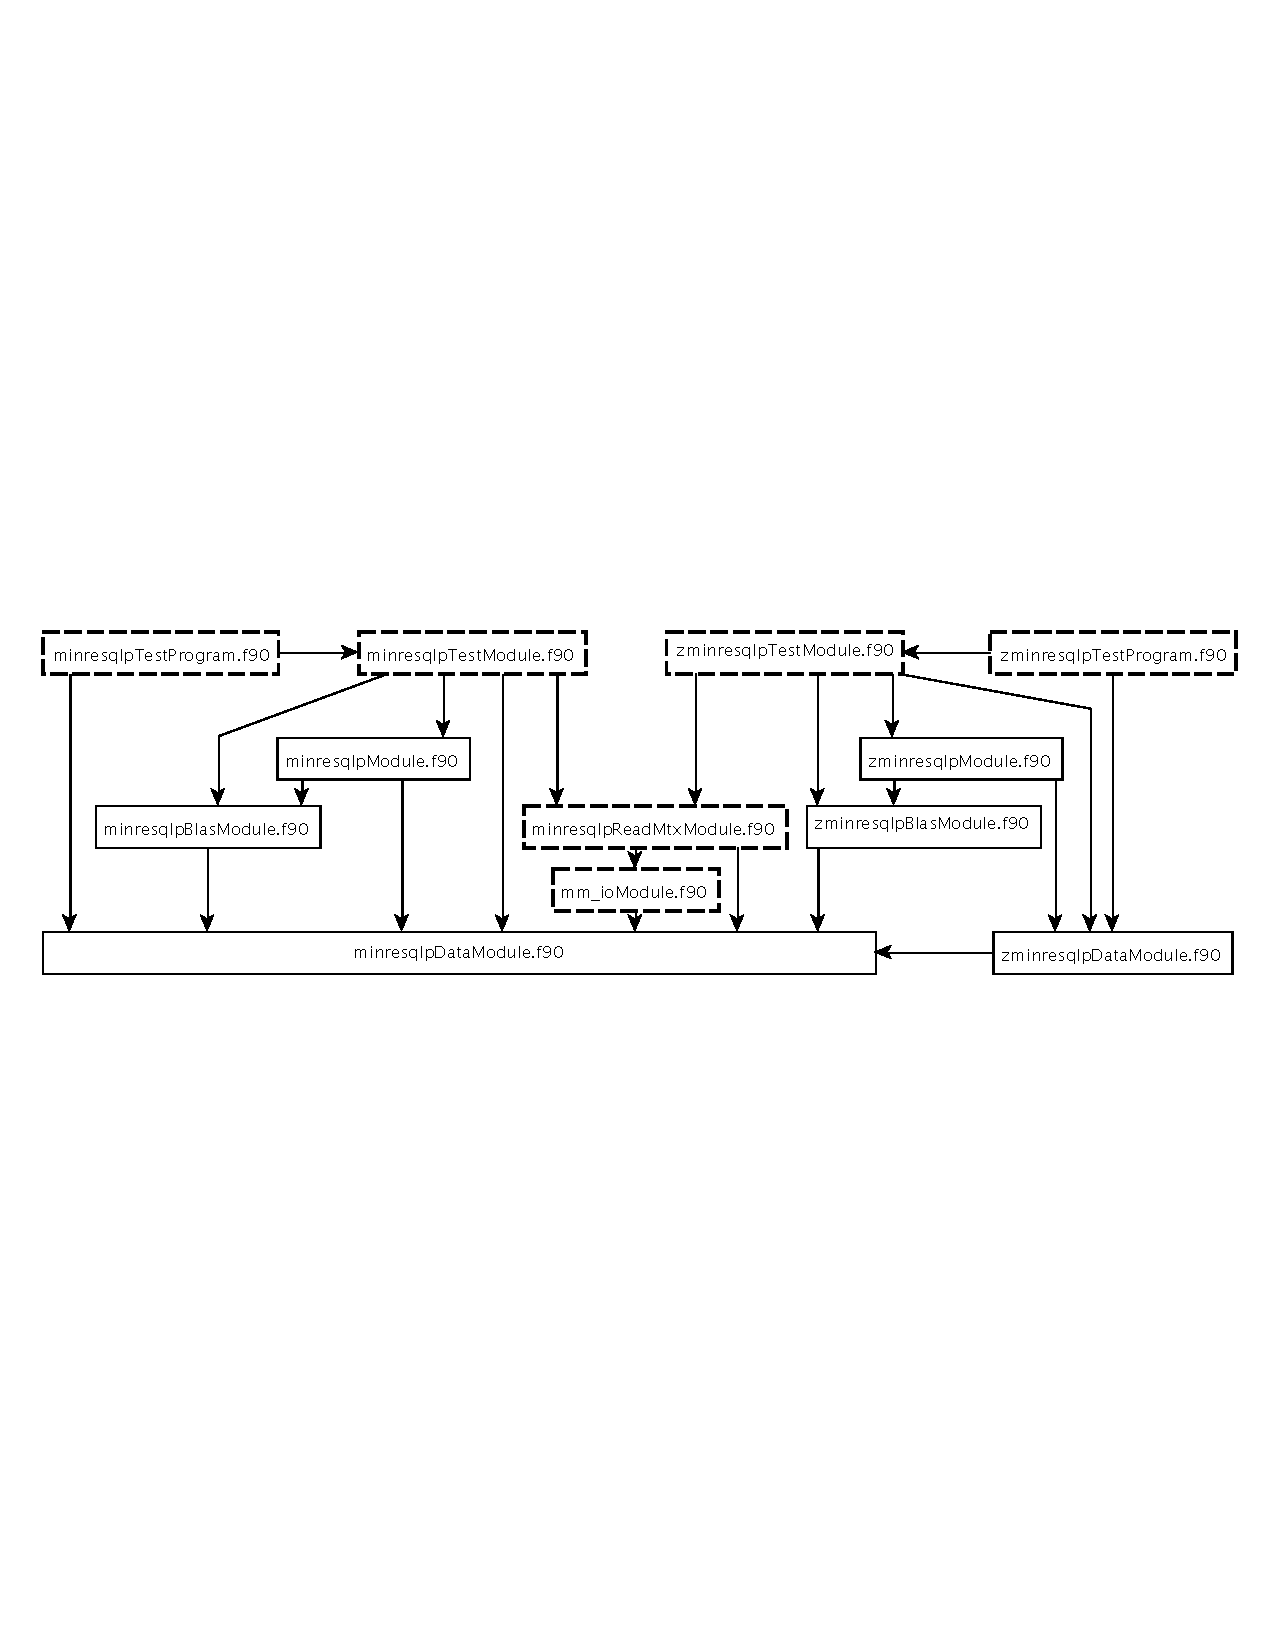
\includegraphics[scale=.6]{f90-program-real-complex-units.pdf}
\caption{FORTRAN~90 source files and their dependencies. Filenames
  boxed in broken lines are optional, and the corresponding files are
  used mainly for testing and demonstration.}
\label{fig:f90-program-units}
\end{figure}


Our \FORTRAN~90 package contains the following files for symmetric
problems with the first three files forming the core. Their
dependencies are depicted in Figure~\ref{fig:f90-program-units}.
\begin{enumerate}[\upshape 1.]
\item \texttt{minresqlpDataModule.f90}: defines integer and real precision
  and constants used in other modules
\item \texttt{minresqlpBlasModule.f90}: packages \FORTRAN~90
  versions of some BLAS functions \citeA{netlibblas}
\item \texttt{minresqlpModule.f90}: implements \MINRESQLP with
  preconditioning
\item \texttt{mm\_ioModule.f90} and
  \texttt{minresqlpReadMtxModule.f90}: packages subroutines for
  reading Matrix Market files \citeA{MM} adapted from \citeA{mmio}
\item \texttt{minresqlpTestModule.f90}: illustrates how \MINRESQLP can
  call \texttt{Aprod} or \texttt{Msolve} with a short fixed parameter
  list, even if it needs arbitrary other data
\item \texttt{minresqlpTestProgram.f90}: contains the main driver
  program for unit tests
\item \texttt{Makefile}: compiles the \FORTRAN source files via the
  Unix command \texttt{make}
\item \texttt{readme.txt}: contains information about
  software license, other files in the package, and program
  compilation and execution.
\end{enumerate}
The counterparts of these programs for Hermitian problems have the
same filenames prefixed with the letter ``\texttt{z}''.

%%%%%%%%%%%%%%%%%%%%%%%%%%%%%%%%%%%%%%%%%%%%%%%%%%%%%%%%%%%%%%%%%%%%%

\begin{lstlisting}[frame=TB,float,caption=Partial \FORTRAN~90 code listing
of minresqlpDataModule.,label=code:dataModule]
module minresqlpDataModule                                      < \label{dataModule:1} >
 implicit none                                                  < \label{dataModule:2} >

 intrinsic                        ::      selected_real_kind    < \label{dataModule:3} >

 integer,       parameter, public :: dp = selected_real_kind(15) < \label{dataModule:4} >
 real(kind=dp), parameter, public :: zero = 0.0_dp, one = 1.0_dp < \label{dataModule:5} >
end module minresqlpDataModule
\end{lstlisting}

%%%%%%%%%%%%%%%%%%%%%%%%%%%%%%%%%%%%%%%%%%%%%%%%%%%%%%%%%%%%%%%%%%%%%
 
\begin{lstlisting}[frame=TB,float,caption=Partial code listing of
                   subroutine MINRESQLP in minresqlpModule.,
                   label=code:minresqlpModule,texcl]
module minresqlpModule                                          <\label{minresqlpModule:1}>
 use  minresqlpDataModule, only : dp, one, zero                 <\label{minresqlpModule:2}>
 use  minresqlpBlasModule, only : dnrm2, ddot

 implicit none                                                  <\label{minresqlpModule:3}>

 public   :: MINRESQLP, SYMORTHO                                <\label{minresqlpModule:4}>
contains
  subroutine MINRESQLP(                                        &<\label{minresqlpModule:5}>
             n, Aprod, b, shift, Msolve, disable, nout,        &<\label{minresqlpModule:6}>
             itnlim, rtol, maxxnorm, trancond, Acondlim,       &<\label{minresqlpModule:7}>
             x, istop, itn, rnorm, Arnorm, xnorm, Anorm, Acond )<\label{minresqlpModule:8}>
                      
   <\label{minresqlpModule:8.5}>! Inputs
   integer(ip), intent(in)             :: n                     <\label{minresqlpModule:9}>
   real(dp),    intent(in)             :: b(n)                  <\label{minresqlpModule:10}>
   integer(ip), intent(in), optional   :: itnlim, nout          <\label{minresqlpModule:11}>
   logical,     intent(in), optional   :: disable               <\label{minresqlpModule:12}>
   real(dp),    intent(in), optional   :: shift                 <\label{minresqlpModule:13}>
   real(dp),    intent(in), optional   :: rtol, maxxnorm, trancond, Acondlim<\label{minresqlpModule:14}>
  
  <\label{minresqlpModule:14.1}>! Outputs                                                  
   real(dp),    intent(out)            :: x(n)                  <\label{minresqlpModule:14.2}>
   integer(ip), intent(out), optional  :: istop, itn            <\label{minresqlpModule:14.3}>
   real(dp),    intent(out), optional  :: rnorm, Arnorm, xnorm, Anorm, Acond<\label{minresqlpModule:15}>
  

   interface                                                    <\label{minresqlpModule:16}>
    subroutine Aprod (n,x,y)                    <\label{minresqlpModule:17}>! $y := A x$
      use       minresqlpDataModule             <\label{minresqlpModule:18}>
      integer,  intent(in)    :: n              <\label{minresqlpModule:19}>
      real(dp), intent(in)    :: x(n)           <\label{minresqlpModule:20}>
      real(dp), intent(out)   :: y(n)           <\label{minresqlpModule:21}>
    end subroutine Aprod                        <\label{minresqlpModule:22}>
   <$\vdots$ >                                  <\label{minresqlpModule:23}>
   end interface                                <\label{minresqlpModule:24}>

   intrinsic :: abs, epsilon, sqrt              <\label{minresqlpModule:25}>

   ! Local arrays and variables
   real(dp)  :: r1(n), r2(n), v(n), w(n), wl(n),               &<\label{minresqlpModule:26}>

   <$\vdots$ >                                                  <\label{minresqlpModule:29}>
 end subroutine MINRESQLP                                       <\label{minresqlpModule:30}>
 <$\vdots$ >
end module minresqlpModule                                      <\label{minresqlpModule:31}>
\end{lstlisting}
 
%%%%%%%%%%%%%%%%%%%%%%%%%%%%%%%%%%%%%%%%%%%%%%%%%%%%%%%%%%%%%%%%%%%%%

\begin{lstlisting}[frame=TB,float,caption=Partial code listing of
                   minresqlpTestModule.,label=code:testModule,texcl]
module minresqlpTestModule                            <\label{testModule:1}>
  use  minresqlpDataModule, only : dp                 <\label{testModule:2}>
  use  minresqlpModule,     only : MINRESQLP          <\label{testModule:3}>

  implicit none                                       <\label{testModule:4}>

  public   :: minresqlptest                           <\label{testModule:5}>
  private  :: Aprod, Msolve                           <\label{testModule:6}>

<\label{testModule:7}>  ! DYNAMIC WORKSPACE DEFINED HERE.
<\label{testModule:8}>  ! It is allocated in minresqlptest and used by Aprod or Msolve.

  real(dp), allocatable :: d(:)   <\label{testModule:9}>!\upshape Defines diagonal matrix $D$.
  real(dp)              :: Ashift <\label{testModule:10}>!\upshape Shift diagonal elements of $D$ in Msolve.
  real(dp)              :: Mpert  <\label{testModule:11}>!\upshape Perturbation to D in Msolve
                                  <\label{testModule:12}>!\upshape to avoid having an exact preconditioner.
contains                                                       <\label{testModule:14}>
  subroutine Aprod(n,x,y)                                      <\label{testModule:15}>

    integer,  intent(in)    :: n                               <\label{testModule:16}>
    real(dp), intent(in)    :: x(n)                            <\label{testModule:17}>
    real(dp), intent(out)   :: y(n)                            <\label{testModule:18}>

    integer  :: i                                              <\label{testModule:19}>

    do i = 1, n                                                <\label{testModule:20}>
       y(i) = d(i)*x(i)                                        <\label{testModule:21}>
    end do                                                     <\label{testModule:22}>

  end subroutine Aprod                                         <\label{testModule:23}>

< $\vdots$ >                                                   <\label{testModule:24}>

  subroutine minresqlptest( n, precon, shift, pertM, nout )    <\label{testModule:25}>
  < $\vdots$ >
   call MINRESQLP(n, Aprod, b, shift, Msolve, disable,    &<\label{testModule:26}>
        nout, itnlim, rtol, maxxnorm, trancond, Acondlim, &<\label{testModule:27}>
        x, istop, itn, rnorm, Arnorm, xnorm, Anorm, Acond )<\label{testModule:29}>
                
  < $\vdots$ >                                                 <\label{testModule:30}>
  end subroutine minresqlptest                                 <\label{testModule:31}>
end module minresqlpTestModule
\end{lstlisting}

%%%%%%%%%%%%%%%%%%%%%%%%%%%%%%%%%%%%%%%%%%%%%%%%%%%%%%%%%%%%%%%%%%%%%

We review and step through the code in the following subsections. The
line numbers in Listings~\ref{code:dataModule}--\ref{code:testModule}
are used for reference only and do not correspond to actual line
numbers in the source code.  The vertical dots in
Listing~\ref{code:minresqlpModule} lines~\ref{minresqlpModule:23} and
\ref{minresqlpModule:29} indicate omitted code of one or more lines.
We also note that \FORTRAN~90 keywords are displayed in bold in the
listings, and that comments are marked with exclamation marks in
italics.

\begin{comment}
\subsection{Explicit Typing}

\FORTRAN~77 program units often use \emph{implicit typing}; for
example, \texttt{IMPLICIT double precision (a-h, o-z)} means that a
variable whose name begins with a letter in the ranges of
\texttt{a}--\texttt{h} or \texttt{o}--\texttt{z} is by default to be
of type \texttt{real}.  Nowadays it is standard practice to explicitly
declare variable types and we put \texttt{IMPLICIT NONE} near the
beginning of every \FORTRAN~90 program unit to disallow implicit
typing.


\subsection{Parameterized Real Variables}

In \FORTRAN~77, \texttt{real} variables are by default of single
precision.  To have double precision, \texttt{double precision} could
be used in place of \texttt{real}, but it is just one of the many
kinds of real variables that can be defined in \FORTRAN~90. For
instance, \texttt{minresqlpDataModule} in
Listing~\ref{code:dataModule} line~\ref{dataModule:5} defines the
integer constant \texttt{dp = selected\_real\_kind(15)}, where
\texttt{selected\_real\_kind} is an intrinsic function parameterized
by number of significant digits of precision. Then we use \texttt{dp}
to define double-precision constants (e.g., \texttt{0.0\_dp} in
line~\ref{dataModule:5}) and variables by \texttt{real(kind=dp)} or
simply \texttt{real(dp)} in other program units.

To use a different precision, \MINRESQLP{} users can simply edit the
input argument value of \texttt{dp = selected\_real\_kind(15)} in
\texttt{minresqlpDataModule} line~\ref{dataModule:5}.
\end{comment}



\subsection{Overloaded Intrinsic Operators and BLAS Procedures}

For standard vector operations, we simply apply the intrinsic
arithmetic and assignment operators $\pm, \times, =$.  In addition we
adopt a \FORTRAN~90 translation~\citeA{netlibblas-f90} of two external
level-1 BLAS functions \texttt{ddot} and
\texttt{dnrm2}~\citeA{netlibblas} for computing inner products and two
norms of vectors, which take care to avoid undesirable overflow or
underflow.


In \texttt{minresqlpModule}, the line ``\texttt{use
  minresqlpBlasModule}'' can be omitted if the code is already linked
to a BLAS library.


\subsection{Using Modules and Interface and Passing User-Defined
            Subroutines to \texttt{MINRESQLP}}

In our \FORTRAN~90 implementation, we use \emph{modules} instead of
the obsolete \FORTRAN~77 COMMON blocks for grouping programs units and
data together and controlling their availability to other program
units. A module can use \texttt{public} data and subroutines from
other modules (by declaring an \emph{interface} block), share its own
\texttt{public} data and subroutines with other program units, and
hide its own \texttt{private} data and subroutines from being used by
other program units. We can also use modules to package procedures.

In Listing~\ref{code:minresqlpModule}, line~\ref{minresqlpModule:2},
module \texttt{minresqlpModule} uses the external \texttt{public}
constant \texttt{dp} from \texttt{minresqlpDataModule}. From
line~\ref{minresqlpModule:5} onwards, \texttt{minresqlpModule} defines
a \texttt{public} subroutine \texttt{MINRESQLP}, where we implement
\MINRESQLP{} in Algorithm~\ref{algo-pminresqlp}.

A \FORTRAN subroutine may have multiple and optional input and output
arguments, which transfer information to and from a calling program.
\texttt{MINRESQLP} has a total of 20 arguments (see
lines~\ref{minresqlpModule:5}-\ref{minresqlpModule:8}). The data types
and \texttt{intent} of these arguments are declared in
lines~\ref{minresqlpModule:9}-\ref{minresqlpModule:15}. For example,
the first argument \texttt{n} in line~\ref{minresqlpModule:9} is an
input integer, whereas \texttt{x(n)} in
line~\ref{minresqlpModule:14.2} is an output $n$-vector of double
precision.

Two input arguments \texttt{Aprod} and \texttt{Msolve} are external
user-defined subroutines (Listing~\ref{code:testModule},
lines~\ref{testModule:6} and \ref{testModule:15}-\ref{testModule:24})
being passed into \texttt{MINRESQLP} as inputs---we recommend they be
\texttt{private} for data integrity. The subroutine \texttt{Aprod}
defines the matrix $A$ as an operator (in
Algorithm~\ref{algo-pminresqlp}, line~8). For a given vector $x$, the
\FORTRAN statement \texttt{call Aprod(n, x, y)} must return the
product $y=Ax$ without altering the vector $x$. The subroutine
\texttt{Msolve} is optional, and it defines a symmetric
positive-definite matrix as an operator $M$ that serves as a
preconditioner (line~10 in Algorithm~\ref{algo-pminresqlp}).  For a
given vector $y$, the \FORTRAN statement \texttt{call MSolve(n, y, x)}
must solve the linear system $Mx=y$ without altering the vector $y$.
To provide the compiler the necessary information about these
\texttt{private} subroutines defined in \texttt{minresqlpTestModule},
an \texttt{interface} block in subroutine \texttt{MINRESQLP} is
declared (lines~\ref{minresqlpModule:16}-\ref{minresqlpModule:24} in
Listing~\ref{code:minresqlpModule}), which essentially replicates the
headers of \texttt{Aprod} and \texttt{Msolve} in
\texttt{minresqlpTestModule}
(lines~\ref{testModule:15}-\ref{testModule:24} in
Listing~\ref{code:testModule}).

\texttt{MINRESQLP} is called by the public routine
\texttt{minresqlptest} defined in module \texttt{minresqlpTestModule}
(see lines~\ref{testModule:5}, \ref{testModule:25}-\ref{testModule:31}
in Listing~\ref{code:testModule}).  Since \texttt{MINRESQLP} is public
(Listing~\ref{code:minresqlpModule}, line~\ref{minresqlpModule:4}),
\texttt{minresqlpTestModule} can simply \texttt{use} it
(Listing~\ref{code:testModule}, line~\ref{testModule:3}).  We have not
listed details of \texttt{minresqlptest}, but it calls
\texttt{MINRESQLP} with \texttt{Aprod} and \texttt{Msolve} passed as
parameters (Listing~\ref{code:testModule}, line~\ref{testModule:26}).

We note that subroutine arrays and variables such as \texttt{r1(n)} in
Listing~\ref{code:minresqlpModule}, line~\ref{minresqlpModule:26}, and
\texttt{i} in Listing~\ref{code:testModule}, line~\ref{testModule:19},
are by default private and not accessible to other program units.  In
contrast, module arrays and variables are by default public and
accessible to other program units. We have marked \texttt{d(:),
  Ashift, Mpert} as \texttt{private} in Listing~\ref{code:testModule},
lines~\ref{testModule:9}--\ref{testModule:11}, in order to make them
accessible to only the subroutines \texttt{minresqlptest},
\texttt{Aprod}, and \texttt{Msolve} in the containing module but not
outside.

To summarize, we have described and provided a pattern that allows
\MINRESQLP users to solve different problems by simply editing
\texttt{minresTestModule} (and possibly the main program
\texttt{minresTestProgram}, which calls \texttt{minresqlptest}).
Users do not need to change \texttt{MINRESQLP} as long as the header
of subroutines \texttt{Aprod} and \texttt{Msolve} stay the same in
\texttt{minresTestModule}. If necessary, local arrays or variables
such as \texttt{d(:)} can be used instead of additional input
arguments to define these operators.  In this way, users can make the
data $A$ and $M$ known to \texttt{MINRESQLP} but hidden and thus
secure from other programs.


Our design spares users from implementing \textit{reverse communication},
in which the solver would return control to the calling program whenever
\texttt{Aprod} or \texttt{Msolve} were to be invoked.  (While reverse
communication is widely used in scientific computing with \FORTRAN~77,
the resulting code usually appears formidable and unrecognizable
from the original pseudocode; see \cite{DEK95} and \cite{OS} for two
examples of \CG and numerical integration coded in \FORTRAN~77 and 90,
respectively.)  Our \MINRESQLP implementation achieves the purpose
of reverse communication while preserving code readability and thus
maintainability. The \FORTRAN~90 module structure allows a user's $Ax$
products and $Mx=y$ solves to be implemented outside \MINRESQLP in the
same way that \MATLAB's function handles operate.


\subsection{Unit Testing}

Unit testing is an important software development strategy that cannot
be overemphasized, especially in the scientific computing
communities. Unit testing usually consists of multiple small and fast
but specific and illuminating test cases that check whether the code
behaves as designed.  Software development is incremental, and errors
(also known as bugs) are often found over time. Adding new
functionalities or fixing errors often breaks the code for some
earlier successful test cases. It is therefore critical to expand the
test cases and to ensure that all unit tests are executed with
expected results every time a key program unit is updated.

In our development of \FORTRAN~90 \MINRESQLP, we have created a suite
of $117$ test cases including singular matrices representative of
real-world applications~\cite{FSJSU,DH11}.  The test program outputs
results to \texttt{MINRESQLP.txt}. If users need to modify subroutine
\texttt{MINRESQLP}, they can run these test cases and search for the
word ``appear'' in the output file to check whether all tests are
reported to be successful.  For more sophisticated unit testing
frameworks employed in large-scale scientific software development,
see~\cite{OTL08}.


\subsection{Miscellaneous Issues}

The complex program units for Hermitian linear systems and LS problems
are similar to the real ones, and thus we will not go into detail.
Many variables of type \texttt{real(dp)} are changed to
\texttt{complex(dp)}.

To use a different precision throughout the program units, \MINRESQLP
users can simply edit the input argument value of \texttt{dp} in
\texttt{minresqlpDataModule}, line~\ref{dataModule:4}.

In the main subroutine \texttt{MINRESQLP}, we provide a logical
parameter \texttt{debug} as a diagnostic tool; when it is true,
variable values are printed to the standard output.


\section{INPUTS, OUTPUTS, AND NUMERICAL EXAMPLES}

Subroutine \texttt{MINRESQLP} contains the core implementation of
\MINRESQLP and has $12$ input parameters documented in the code as
well as in Table~\ref{table-input}.  It uses seven local $n$-vectors
and returns a computed solution \texttt{x} as one of the eight
outputs. Mandatory inputs are $n$, \texttt{Aprod}, and $b$.  All
outputs other than $x$ are optional. If an input is optional,
\MINRESQLP prescribes a default value.  It is well known that careful
choice of parameter values is critical in the convergence behavior of
iterative solvers.   While the default
parameter values in \MINRESQLP work well in most tests, they may need
to be fine-tuned by trial and error, and for some applications it may
be worthwhile to implement full or partial reorthogonalization of the
Lanczos vectors \cite{S84b}.

 
\begin{center}
\begin{longtable}{ll}  %%% Table III
%
\caption{Input parameters in subroutine MINRES-QLP.} 
\label{table-input}
%
\\[.1ex] \hline
\\[.0ex] \bfseries Input & \bfseries Definition
\\[1ex]  \hline
\\[0.5ex]
\endfirsthead
%
\multicolumn{2}{c}%
{{\tablename\ \thetable{}: Input parameters in MINRES-QLP (continued).}} 
\\
\\[.1ex] \hline
\\[.0ex] \bfseries Input & \bfseries Definition
\\[1ex]  \hline
\\[0.5ex]
\endhead
%
                $n$      & The dimension of the symmetric 
                   matrix or operator $A$.
\\[2ex] $b(n)$   & The right-hand-side vector $b$.
\\[2ex] \texttt{Aprod} 
                 & An external subroutine defining 
                   the matrix $A$. For a given vector $x$, 
\\               & the statement \texttt{call Aprod ( n, x, y )} 
                   must return the product 
\\               & $y = Ax$ without altering the vector $x$. 
                   An extra call of \texttt{Aprod} is  
\\               & used to check if $A$ is symmetric.  
                   The program calling \MINRESQLP{} 
\\               & must declare \texttt{Aprod} to be external.
\\[2ex] \texttt{Msolve} 
                 & An optional external subroutine 
                   defining a preconditioner $M$, which
\\               &  should approximate $A - \mathit{shift} I$ 
                   in some sense. If present, $M$ must 
\\               & be symmetric positive definite. For a given 
                   vector $x$, the statement
\\               & \texttt{call Msolve( n, x, y )} must 
                   solve the linear system $My = x$
\\               & without altering the vector $x$. 
                   In general, $M$ should be chosen 
\\               & so that $\tilde{A} \equiv  M^{-\myhalf} \Abar M^{-\myhalf}$ 
                   has more clustered eigenvalues. If $\Abar$  
\\               & is positive definite, $\tilde{A}$ 
                   would ideally be close to a multiple of $I$.
\\               & If $\Abar$ is indefinite, $\tilde{A}$ might be
                   close to a multiple of \texttt{diag}($I$ \; $-I$).
\\               & If $M$ is absent, no preconditioner is applied.
\\[2ex] $\mathit{shift}$ 
                 & Should be zero if the system $Ax = b$ is to be
                   solved. Otherwise, it
\\               & could be an approximation to an eigenvalue of $A$,
                   such as the
\\               & Rayleigh quotient $(b\T Ab) / (b\T b)$
                   corresponding to the vector $b$.
\\               & If $b$ is sufficiently like an eigenvector
                   corresponding to an
\\               & eigenvalue near $\mathit{shift}$, then the
                   computed $x$ may have very large
\\               & components. When normalized, $x$ may be closer to an eigenvector
\\               & than $b$. Default value is 0.
\\[2ex] $\mathit{nout}$ 
                 & A file number. The calling program must 
                   open a file for  
\\               & output using for example:  
\\               & \texttt{open(nout, file=`MINRESQLP.txt', status=`unknown')}. 
\\               & If $\mathit{nout} > 0$, 
                   a summary of the iterations will be printed on unit
\\               & $\mathit{nout}$. If $\mathit{nout}$ is absent
                   or the file associated with $\mathit{nout}$ is not
\\               & opened properly, results will be written to 
                   \texttt{MINRESQLP\_tmp.txt}.
\\               & Default value is 10.
\\[2ex] $\mathit{itnlim}$
                 & An upper limit on the number of iterations. 
                   Default to $4n$.
\\[2ex] $\mathit{rtol}$
                 & A user-specified tolerance. \MINRESQLP{}
                   terminates if it appears 
\\               & that $\norm{\rbar}$ is smaller than $\mathit{rtol}
                   (\norm{\Abar} \norm{\xbar}+\norm{b})$, where
                   $\rbar = \bbar - \Abar \xbar$,
\\               & or that 
                   $\norm{\Abar \rbar}$ is smaller than
                   $\mathit{rtol} \norm{\Abar} \norm{\rbar}$.
\\               & If $\mathit{shift} = 0$ and \texttt{Msolve} is absent, 
                   \MINRESQLP{} terminates if  
\\               & $\norm{r}$ is smaller than $\mathit{rtol} (\norm{A} \norm{x}
                   + \norm{b})$, where $r=b-Ax$,  
\\               & or if $\norm{Ar}$ is smaller than 
                   $\mathit{rtol} \norm{A} \norm{r}$.
                   Default to  $\varepsilon$.
\\[2ex] $\mathit{maxxnorm}$
                 & An upper bound on $\norm{x}$. Default value is $10^7$.
\\[2ex] $\mathit{Acondlim}$
                 & An upper bound on $\mathit{Acond}$, an estimate of
                   $\cond(A)$. 
\\               & Default value is $10^{15}$.
\\[2ex] $\mathit{trancond}$
                 & If $\mathit{trancond} > 1$, a switch is made from
                   \MINRES iterations 
\\               & to \MINRESQLP iterations when $\mathit{Acond} \ge
                   \mathit{trancond}$.
\\               & If $\mathit{trancond} = 1$, all iterations will be
                   \MINRESQLP{} iterations.
\\               & If $\mathit{trancond} = \mathit{acondlim}$, all
                   iterations will be conventional
\\               & \MINRES{} iterations (which are slightly cheaper).
\\               & Default value is $10^7$.
\\[1.5ex] \hline
\end{longtable}
\end{center}



We use two small examples to illustrate the output of
\texttt{MINRESQLP}.  \cite[Chapter 4]{C06} or
\cite[Section 8]{CPS11} give more significant numerical examples.

Table~\ref{small-eg} compares the \MINRES solution to the \MINRESQLP
solution for the small problem $Ax \approx b$, where
$A=\diag\left(\bmat{1, \dots, 10, 0}\right)$ and $b$ is a vector of
all ones. Clearly, all but the last components are the same (in
general, all components are different), and \MINRESQLP gives the
minimum-length solution, whereas \MINRES returns a minimum residual
solution.


\begin{center}
\begin{longtable}{c c}
\caption{MINRES and MINRES-QLP solutions of $Ax \approx e$,
         where $A = \diag[1, \dots, 10, 0]$.}
\label{small-eg}
\\ \hline
\\ \bfseries MINRES         &  \qquad \bfseries MINRES-QLP
\\[1.5ex] \hline
\vspace{.00in}
\endhead
     1.000000000000001 & \qquad    1.000000000000000
\\   0.500000000000001 & \qquad    0.500000000000001
\\   0.333333333333333 & \qquad    0.333333333333333
\\   0.250000000000001 & \qquad    0.250000000000001
\\   0.199999999999999 & \qquad    0.199999999999999
\\   0.166666666666667 & \qquad    0.166666666666667
\\   0.142857142857143 & \qquad    0.142857142857143
\\   0.125000000000000 & \qquad    0.125000000000000
\\   0.111111111111111 & \qquad    0.111111111111111
\\   0.100000000000000 & \qquad    0.100000000000000
\\   2.928968253967685 & \qquad    0.000000000000000
\\[1.5ex]\hline
\end{longtable}
\end{center}

The program produces printed output on file \texttt{nout}, if that
parameter is positive. This is illustrated below,
in which another least-squares problem (Ex.~21 in
\texttt{minresqlpTestProgram}) is solved: $\min \norm{x}$ such that $x
\in \arg\min\norm{\diag\bmat{d,0,0}x - b}$, where
$d\equiv\bmat{\frac{1}{50},\frac{2}{50},\dots,\frac{48}{50}}\T$ and $b
\equiv \bmat{d,1,1}\T .* \bmat{50:-1:3,1,1}\T$, where $.*$ indicates
elementwise multiplication. No preconditioner is applied, and shift
$\sigma = 0$.

Notice that the rightmost column of the 39th iteration is marked with
``\texttt{P}'', which indicates that the program switches from \MINRES{} phase
to \MINRESQLP{} phase since $\mathcal{A}_{39} \approx 1.81 \times 10^7
> \mathit{trancond} = 10^7$.  Even though the last line in the output
reports that \MINRESQLP{} has to stop at iteration 46 because
$\norm{x_{47}} > \mathit{maxxnorm}$, the algorithm appears to be
successful because the relative error in $x_{46}$ is merely $2.8
\times 10 ^{-13}$.

%\newpage 
\vspace{-0.1in}
\begin{center}
{\footnotesize
\begin{ttlongtable}{r@{\,\,}r@{\,\,}r@{\,\,}r@{\,\,}r@{\,\,}
                    r@{\,\,}r@{\,\,}r@{\,\,}r@{\,\,}r@{}}
\\[-1ex]\hline
\\\multicolumn{2}{l}{Enter MINRES-QLP.    }&\multicolumn{8}{l}{Solution of symmetric  Ax = b}
\\\multicolumn{2}{l}{n      =     50      }&\multicolumn{3}{l}{||b||    =  6.78E+01  }& \multicolumn{4}{l}{precon = F}
\\\multicolumn{2}{l}{itnlim =    200      }&\multicolumn{3}{l}{rtol     =   2.22E-16 }& \multicolumn{4}{l}{shift  = 0.00E+00}
\\\multicolumn{2}{l}{maxxnorm =  1.00E+07 }&\multicolumn{3}{l}{Acondlim =   1.00E+15  }& \multicolumn{4}{l}{trancond =   1.00E+07}
\\
\\iter  & x(1)             &  xnorm   &  rnorm   &  Arnorm  & Compatible &   LS     &  norm(A) &  cond(A)
\\   0  & 0.0000000000E+00 & 0.00E+00 & 6.78E+01 & 3.69E+01 & 1.00E+00   & 1.00E+00 & 0.00E+00 & 1.00E+00  
\\   1  & 1.7180943901E+00 & 1.16E+02 & 2.40E+01 & 1.09E+01 & 1.83E-01   & 6.94E-01 & 5.44E-01 & 1.00E+00  
\\   2  & 3.8644538109E+00 & 1.53E+02 & 1.15E+01 & 4.58E+00 & 6.82E-02   & 6.06E-01 & 6.57E-01 & 1.70E+00  
\\   3  & 6.3954779963E+00 & 1.72E+02 & 6.51E+00 & 2.30E+00 & 3.60E-02   & 5.37E-01 & 6.57E-01 & 2.27E+00  
\\   4  & 9.2579303917E+00 & 1.83E+02 & 4.16E+00 & 1.29E+00 & 2.21E-02   & 4.74E-01 & 6.57E-01 & 2.94E+00  
\\   5  & 1.2389816033E+01 & 1.90E+02 & 2.94E+00 & 7.91E-01 & 1.52E-02   & 4.10E-01 & 6.57E-01 & 3.74E+00  
\\   6  & 1.5722893791E+01 & 1.95E+02 & 2.28E+00 & 5.14E-01 & 1.16E-02   & 3.43E-01 & 6.57E-01 & 4.78E+00  
\\   7  & 1.9185796048E+01 & 2.00E+02 & 1.91E+00 & 3.50E-01 & 9.61E-03   & 2.79E-01 & 6.57E-01 & 6.20E+00  
\\   8  & 2.2706980590E+01 & 2.03E+02 & 1.71E+00 & 2.48E-01 & 8.47E-03   & 2.21E-01 & 6.57E-01 & 8.20E+00  
\\   9  & 2.6217158315E+01 & 2.07E+02 & 1.59E+00 & 1.81E-01 & 7.81E-03   & 1.73E-01 & 6.57E-01 & 1.10E+01  
\\      &                  &          &          &          &            &          &          &           
\\  10  & 2.9651001936E+01 & 2.10E+02 & 1.52E+00 & 1.36E-01 & 7.39E-03   & 1.36E-01 & 6.57E-01 & 1.50E+01  
\\  20  & 4.9405101158E+01 & 2.71E+02 & 1.41E+00 & 1.08E-02 & 5.76E-03   & 1.16E-02 & 6.57E-01 & 1.92E+02  
\\  30  & 4.9999971981E+01 & 3.22E+02 & 1.41E+00 & 6.37E-05 & 5.06E-03   & 6.86E-05 & 6.57E-01 & 1.18E+04  
\\  39  & 5.0000000000E+01 & 3.53E+02 & 1.41E+00 & 2.09E-08 & 4.72E-03   & 2.25E-08 & 6.57E-01 & 1.81E+07 & P
\\      &                  &          &          &          &            &          &          &
\\  40  & 5.0000000000E+01 & 3.56E+02 & 1.41E+00 & 6.60E-09 & 4.69E-03   & 7.10E-09 & 6.57E-01 & 5.29E+07
\\  45  & 5.0000000000E+01 & 3.76E+05 & 1.41E+00 & 5.53E-07 & 5.73E-06   & 5.95E-07 & 6.57E-01 & 2.01E+11
\\  46  & 5.0000000000E+01 & 2.07E+02 & 1.41E+00 & 5.86E-07 & 5.73E-06   & 6.30E-07 & 6.57E-01 & 2.01E+11
\\
\\\multicolumn{2}{l}{Exit  MINRES-QLP.   }&\multicolumn{3}{l}{istop =  12             }&\multicolumn{4}{l}{itn   =      46    }
\\\multicolumn{2}{l}{Exit  MINRES-QLP.   }&\multicolumn{3}{l}{Anorm =  6.5701E-01     }&\multicolumn{4}{l}{Acond =  2.0123E+11}
\\\multicolumn{2}{l}{Exit  MINRES-QLP.   }&\multicolumn{3}{l}{rnorm =  1.4142E+00     }&\multicolumn{4}{l}{Arnorm = 1.2149E-05}
\\\multicolumn{2}{l}{Exit  MINRES-QLP.   }&\multicolumn{3}{l}{xnorm =  2.0717E+02     }
\\\multicolumn{2}{l}{Exit  MINRES-QLP.   }&\multicolumn{8}{l}{xnorm has exceeded maxxnorm or will exceed it next iteration.}
\\
\\\hline
{\addtocounter{table}{-1}} % Without this line, the next table would be enumerated as Table VI (six) rather than Table V (five).
\end{ttlongtable}
}
\end{center}

\vspace{-2\baselineskip}

The items printed at the $k$th iteration are listed and explained
in the source code. For simplicity we assumed   no
preconditioner below; when there is one, we simply replace $\Abar$ and
$r_k$, respectively, with $\tilde{A}$ and $\bar{r}_k$ as defined in
Section~\ref{sect-precond} and Algorithm~\ref{algo-pminresqlp}.

\begin{center}
\vspace{-.1in}
\begin{longtable}{l l} %%% Table V
\caption{Items printed at the $k$th iteration.} \label{table-printed-outputs}
%
\\[0ex]\hline
\\ \bfseries Label       &  \bfseries Definition
\\[1ex]\hline
\\[0.2ex]
\endfirsthead
%
\multicolumn{2}{c}%
{{\tablename\ \thetable{}: Items printed at the $k$th iteration (continued).}} 
\\
\\[0ex]\hline
\\ \bfseries Label       &  \bfseries Definition
\\[1ex]\hline
\\[0.2ex]
\endhead
        $\mathit{iter}$  &  The iteration number $k$.  Results are
                            always printed for the first
\\                       &  10 iterations and the last. Intermediate
                            results are printed
\\                       &  every 10th iteration. 
\\[2ex] $x(1)$           &  The value of the first element of the
                            approximate solution $x_k$.
\\[2ex] $\mathit{xnorm}$ &  $\norm{x_k}$.
\\[2ex] $\mathit{rnorm}$ &  $\norm{r_k}$.
\\[2ex] $\mathit{Arnorm}$&  $\norm{\Abar r_k}$.
\\[2ex] $\mathit{Compatible}$
                         &  A dimensionless quantity that should
                            converge to zero if and
\\                       &  only if $\Abar x=b$ is compatible. It is
                            an estimate of
\\                       &  $\norm{r_k}/(\norm{\Abar}\norm{x_k}+\norm{b})$,
                            which decreases monotonically.
\\[2ex] $\mathit{LS}$    &  A dimensionless quantity that should
                            converge to zero if and
\\                       &  only if the optimum $r_k$ is nonzero. It
                            is an estimate of
\\                       &  $\norm{\Abar r_k}/(\norm{\Abar}\norm{r_k})$,
                            which is usually not monotonic.
\\[2ex] $\mathit{norm(A)}$
                         &  A monotonically increasing underestimate
                            of $\norm{\Abar}$.
\\[2ex] $\mathit{cond(A)}$
                         &  A monotonically increasing underestimate
                            of $\cond(\Abar)$.
\\[2ex]\hline
\end{longtable}
\end{center}

\vspace{-.1in}
The integer output \texttt{istop} takes an initial value of 0; when
the program stops, it takes a positive integer value between 1 to 14
inclusive to signify one of the termination conditions in
Table~\ref{table-stopping-conditions}.
We note that if $\texttt{istop} > 7$, the final $x$ may or may not be
an acceptable solution. On the contrary, when $\texttt{istop} \le 7$,
we can be sure $x_k$ is a good or even an excellent approximate
solution of a given problem.


\begin{center}
\vspace{.1in}
\begin{longtable}{c l} %%% Table VI
\caption{Termination conditions in MINRES-QLP.}
\label{table-stopping-conditions}
%
\\[2ex]\hline \\ \bfseries \texttt{istop}      &  \bfseries Termination Conditions
\\[2ex]\hline
\\[0.5ex]
\endfirsthead
%
\multicolumn{2}{c}%
{{\tablename\ \thetable{}: Termination conditions in MINRES-QLP (continued).}} 
\\
\\[0.5ex]\hline \\ \bfseries \texttt{istop}      &  \bfseries Termination Conditions
\\[1.5ex]\hline
\\[0.5ex]
\endhead
         1 & $\beta_{k+1} < \varepsilon$. Iteration
             $k$ is the final Lanczos step. Rarely occurs.
\\[1.5ex]  2 & $\beta_2 = 0$ in the Lanczos iteration; i.e. the second
             Lanczos vector is zero.
\\           & This means the right-hand-side is very special. If
             there is no
\\           & preconditioner, $b$ is an eigenvector of $A$.
\\           & Otherwise (if $\mathit{precon}$ is true), let $My = b$.
             If shift is zero, $y$ is a solution
\\           & of the generalized eigenvalue problem $Ay = \lambda My$,
             with $\lambda = \alpha_1$ from
\\           & the Lanczos vectors. In general, $(A - \sigma I)x = b$
             has the solution
\\           & $x = (1/\alpha_1) y$, where $My = b$.
\\[1.5ex]  3 & $b = 0$, so the exact solution is $x = 0$. No iterations
             were performed.
\\[1.5ex]  4 & $\norm{\rbar}$ appears to be less than the value
             $\mathit{rtol} (\norm{\Abar} \norm{\xbar} + \norm{b})$; $x$ should
\\           & be an acceptable solution of $\Abar x = b$.
\\[1.5ex]  5 & $\norm{\rbar}$ appears to be less than the value
             $\varepsilon (\norm{\Abar} \norm{\xbar} + \norm{b})$. This means
\\           & that the solution is as accurate as seems reasonable on this machine.
\\[1.5ex]  6 & $\norm{\Abar\rbar}$ appears to be less than the value
             $\mathit{rtol} \norm{\Abar} \norm{\rbar}$; $x$ should be an
\\           & acceptable least-squares solution.
\\[1.5ex]  7 & $\norm{\Abar\rbar}$ appears to be less than the value
             $\varepsilon \norm{\Abar} \norm{\rbar}$. This means that the
\\           & least-squares solution is as accurate as seems reasonable
             on this
\\           & machine.
\\[1.5ex]  8 & The iteration limit was reached before convergence.
\\[1.5ex]  9 & The matrix defined by  \texttt{Aprod} does not appear to
             be symmetric. For
\\           & certain vectors $y = Av$ and $r = Ay$, the products
             $y\T y$ and $r\T v$ differ
\\           & significantly.
\\[1.5ex] 10 & The matrix defined by \texttt{Msolve} does not appear to
             be symmetric.  For
\\           & vectors satisfying $My = v$ and $Mr = y$, the products
             $y\T y$ and $r\T v$
\\           & differ significantly.
\\[1.5ex] 11 & An inner product of the form  $x\T M^{-1} x$ was not
             positive, so the
\\           & preconditioner $M$ does not appear to be positive
             definite.
\\[1.5ex] 12 & $\norm{x}$ has exceeded $\mathit{maxxnorm}$ or will exceed it next iteration.
\\[1.5ex] 13 & $\cond(\Abar)$  has exceeded $\mathit{Acondlim}$ or 0.1/$\varepsilon$, so $\Abar$
             must be very
\\           & ill-conditioned.
\\[1.5ex] 14 & $|\gamma_k^{(4)}| < \varepsilon$. This is probably a
             least-squares problem but residual norms  
\\           &  have not satisfied NRBE conditions.  
\\[1.5ex]\hline
\end{longtable}
\end{center}
\vspace{-1\baselineskip}


\section{AVAILABILITY}

Implementations of \MINRESQLP{} are available in \FORTRAN~90 and
\MATLAB~7.8 from the Systems Optimization Laboratory, Stanford
University \hbox{\citeA{SOL}}, or the first author's homepage
\url{http://home.uchicago.edu/sctchoi/} under the terms of the OSI
Common Public License (CPL) \hbox{\citeA{OSI-CPL}} or the BSD License
\hbox{\citeA{BSD}}.



\begin{acks}
  We thank Christopher Paige for his contribution to the theory of
  \MINRESQLP, including the simplified proof of Theorem 2.2.  We also
  thank Tim Hopkins and David Saunders for testing and running our
  software on the NAG Fortran compiler and the Intel ifort compiler respectively,
  resulting in more robust code. We are grateful to Zhaojun Bai and
  two anonymous reviewers for their patience and constructive
  comments. The first author thanks Jed Brown, Ian Foster, Todd
  Munson, Gail Pieper, Stefan Wild, and Hong Zhang for their feedback,
  interest, and support for this work.  Finally,
  we express our gratitude to the SIAM SIAG/LA 2012 Linear Algebra
  Prize Committee for their favorable consideration of
  \MINRESQLP.
\end{acks}

 

\bibliographystyle{acmtrans}
\bibliography{refs3} %refs3.bib


\vfill
{\small The submitted manuscript has been created by the University of
  Chicago as Operator of Argonne National Laboratory (``Argonne'')
  under Contract DE-AC02-06CH11357 with the U.S. Department of Energy.
  The U.S. Government retains for itself, and others acting on its
  behalf, a paid-up, nonexclusive, irrevocable worldwide license in
  said article to reproduce, prepare derivative works, distribute
  copies to the public, and perform publicly and display publicly, by
  or on behalf of the Government.}

\end{document}
